\documentclass[aspectratio=169,xcolor=table]{beamer}

% Theme settings
\usetheme{Madrid}
\usecolortheme{dolphin}
\setbeamertemplate{navigation symbols}{}  % Remove navigation symbols
\setbeamertemplate{footline}[frame number]
\useoutertheme{miniframes}
\useinnertheme{circles}

% Packages
\usepackage{booktabs}
\usepackage{graphicx}
\usepackage{amsmath}
\usepackage{amssymb}
\usepackage{xcolor}
\usepackage{algorithm}
\usepackage{algorithmic}
\usepackage{tikz}
\usetikzlibrary{arrows,shapes,positioning,shadows,trees,mindmap}
\usepackage{tcolorbox}
\tcbuselibrary{skins}

% Graphics path
\graphicspath{{./}}

% Define custom colors
\definecolor{fuzzygreen}{RGB}{46, 204, 113}
\definecolor{psocolor}{RGB}{52, 152, 219}
\definecolor{adaptivecolor}{RGB}{255, 149, 0}
\definecolor{parallelcolor}{RGB}{255, 87, 51}
\definecolor{islandcolor}{RGB}{199, 0, 57}

% Custom styles for blocks
\setbeamercolor{block title}{bg=blue!30,fg=white}
\setbeamercolor{block body}{bg=blue!10,fg=black}

\setbeamercolor{alerted text}{fg=red!80!black}
\setbeamercolor{example text}{fg=green!60!black}

% Custom command for block styling
\newcommand{\customblock}[2]{%
    \begin{tcolorbox}[
        enhanced,
        colback=blue!5,
        colframe=blue!70,
        arc=2mm,
        fonttitle=\bfseries\large,
        title=#1,
        boxrule=0.5mm,
        drop shadow={opacity=0.15}
    ]
        #2
    \end{tcolorbox}
}

% Title information
\title{Comparative Analysis of Various PSO Algorithms with Fuzzy Logic for Portfolio Optimization}
\subtitle{Performance and Efficiency Evaluation with DJIA Stocks}
\author{Cemal Öztürk}
\institute{Pamukkale University\\ Department of Computer Engineering}
\date{April 17, 2025}

\begin{document}

% Title page
\begin{frame}
  \titlepage
\end{frame}

% Table of contents
\begin{frame}{Outline}
  \tableofcontents
\end{frame}

% Section: Introduction
\section{Introduction}

\begin{frame}{Introduction}
  \begin{tcolorbox}[
    enhanced,
    colback=blue!5,
    colframe=blue!70,
    arc=2mm,
    title=Portfolio Optimization Challenges,
    fonttitle=\bfseries\large,
    boxrule=0.5mm
  ]
    \begin{itemize}
      \item Portfolio optimization is a critical task in financial management
      \item Traditional methods (Markowitz) have limitations in various market conditions
      \item Need for more robust and adaptive optimization algorithms
    \end{itemize}
  \end{tcolorbox}
  
  \vspace{0.3cm}
  
  \begin{tcolorbox}[
    enhanced,
    colback=blue!5,
    colframe=blue!70,
    arc=2mm,
    title=Our Approach,
    fonttitle=\bfseries\large,
    boxrule=0.5mm
  ]
    \begin{itemize}
      \item Evolutionary and swarm intelligence algorithms offer new possibilities
      \item Five algorithms compared with same data and evaluation criteria:
        \begin{itemize}
          \item Genetic Algorithms (GA)
          \item Standard Particle Swarm Optimization (PSO)
          \item Adaptive PSO
          \item Parallel PSO
          \item Island Model PSO
        \end{itemize}
      \item All integrated with a fuzzy logic inference system for objective evaluation
    \end{itemize}
  \end{tcolorbox}
\end{frame}

\begin{frame}{Research Objectives}
  \begin{tcolorbox}[
    enhanced,
    colback=blue!5,
    colframe=blue!70,
    arc=2mm,
    title=Main Goals,
    fonttitle=\bfseries\large,
    boxrule=0.5mm
  ]
    \begin{itemize}
      \item Compare the performance of various optimization algorithms for portfolio management
      \item Evaluate the effectiveness of fuzzy logic in guiding optimization
      \item Assess the speed improvements from parallel processing strategies
      \item Develop more efficient and accurate portfolio optimization techniques
    \end{itemize}
  \end{tcolorbox}
  
  \vspace{0.5cm}
  
  \begin{tcolorbox}[
    enhanced,
    colback=blue!5,
    colframe=blue!70,
    arc=2mm,
    title=Research Questions,
    fonttitle=\bfseries\large,
    boxrule=0.5mm
  ]
    \begin{itemize}
      \item Which algorithm provides the best risk-adjusted returns?
      \item How significant are the speed improvements with parallel implementations?
      \item Does adaptive parameter tuning improve optimization quality?
      \item How do these algorithms perform compared to traditional methods?
    \end{itemize}
  \end{tcolorbox}
\end{frame}

% Section: Methodology
\section{Methodology}

\begin{frame}{Data and Portfolio Construction}
  \begin{columns}
    \begin{column}{0.6\textwidth}
      \begin{tcolorbox}[
        enhanced,
        colback=blue!5,
        colframe=blue!70,
        arc=2mm,
        title=Dataset Description,
        fonttitle=\bfseries\large,
        boxrule=0.5mm
      ]
        \begin{itemize}
          \item Dataset: DJIA 30 component stocks
          \item Period: January 1990 to April 2025
          \item Train/test split: 70\%/30\% (1068/458 days)
          \item Statistical measures:
            \begin{itemize}
              \item Expected returns (annualized)
              \item Covariance matrix
              \item Volatility and Sharpe ratios
            \end{itemize}
          \item Sector information for diversification constraints
        \end{itemize}
      \end{tcolorbox}
    \end{column}
    \begin{column}{0.4\textwidth}
      % Data processing workflow diagram
      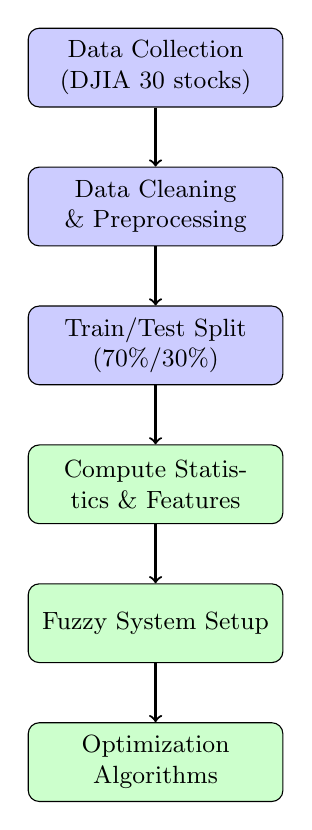
\begin{tikzpicture}[
        node distance=0.75cm,
        box/.style={draw, rectangle, rounded corners, minimum width=3cm, minimum height=1cm, text centered, text width=3cm, font=\small}
      ]
        \node[box, fill=blue!20] (data) {Data Collection (DJIA 30 stocks)};
        \node[box, fill=blue!20, below=of data] (clean) {Data Cleaning \& Preprocessing};
        \node[box, fill=blue!20, below=of clean] (split) {Train/Test Split (70\%/30\%)};
        \node[box, fill=green!20, below=of split] (stats) {Compute Statistics \& Features};
        \node[box, fill=green!20, below=of stats] (fuzzy) {Fuzzy System Setup};
        \node[box, fill=green!20, below=of fuzzy] (opt) {Optimization Algorithms};
        
        \draw[->,thick] (data) -- (clean);
        \draw[->,thick] (clean) -- (split);
        \draw[->,thick] (split) -- (stats);
        \draw[->,thick] (stats) -- (fuzzy);
        \draw[->,thick] (fuzzy) -- (opt);
      \end{tikzpicture}
    \end{column}
  \end{columns}
\end{frame}

\begin{frame}{Data Processing Pipeline}
  \centering
  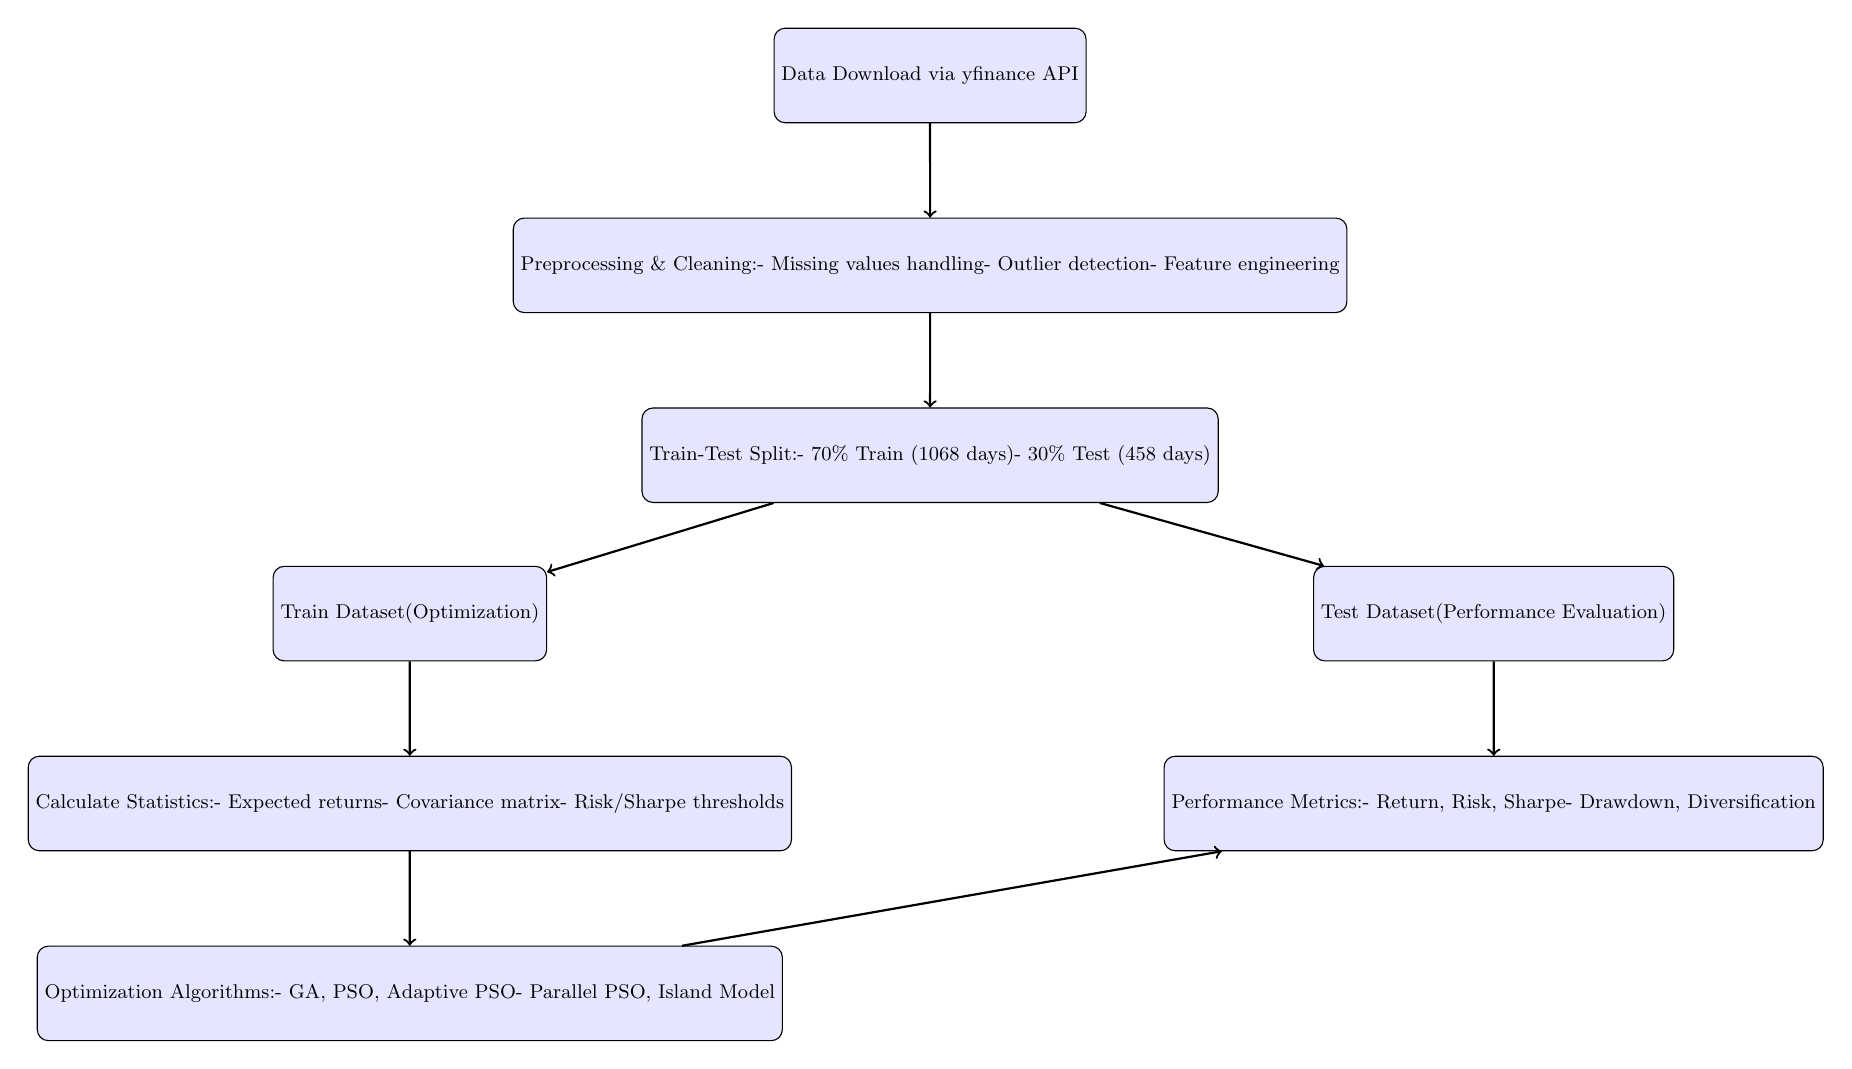
\begin{tikzpicture}[
    node distance = 1.5cm,
    scale=0.8, transform shape,
    box/.style={rectangle, draw, rounded corners, fill=blue!10, minimum width=4cm, minimum height=1.5cm, text centered, font=\small}
  ]
    % Nodes
    \node[box] (download) {Data Download via yfinance API};
    \node[box, below=of download] (preprocess) {Preprocessing \& Cleaning:\\- Missing values handling\\- Outlier detection\\- Feature engineering};
    \node[box, below=of preprocess] (split) {Train-Test Split:\\- 70\% Train (1068 days)\\- 30\% Test (458 days)};
    
    \node[box, below right=1cm and 1.5cm of split] (test) {Test Dataset\\(Performance Evaluation)};
    \node[box, below left=1cm and 1.5cm of split] (train) {Train Dataset\\(Optimization)};
    
    \node[box, below=of train] (stats) {Calculate Statistics:\\- Expected returns\\- Covariance matrix\\- Risk/Sharpe thresholds};
    
    \node[box, below=of stats] (optim) {Optimization Algorithms:\\- GA, PSO, Adaptive PSO\\- Parallel PSO, Island Model};
    
    \node[box, below=of test] (eval) {Performance Metrics:\\- Return, Risk, Sharpe\\- Drawdown, Diversification};
    
    % Arrows
    \draw[->, thick] (download) -- (preprocess);
    \draw[->, thick] (preprocess) -- (split);
    \draw[->, thick] (split) -- (train);
    \draw[->, thick] (split) -- (test);
    \draw[->, thick] (train) -- (stats);
    \draw[->, thick] (stats) -- (optim);
    \draw[->, thick] (optim) -- (eval);
    \draw[->, thick] (test) -- (eval);
  \end{tikzpicture}
\end{frame}

\begin{frame}{Fuzzy Logic System Overview}
  \begin{columns}
    \begin{column}{0.5\textwidth}
      \begin{tcolorbox}[
        enhanced,
        colback=blue!5,
        colframe=blue!70,
        arc=2mm,
        title=Fuzzy Inference System Components,
        fonttitle=\bfseries\large,
        boxrule=0.5mm
      ]
        \begin{itemize}
          \item Input variables:
            \begin{itemize}
              \item Risk (portfolio volatility)
              \item Sharpe ratio (risk-adjusted return)
            \end{itemize}
          \item Membership functions:
            \begin{itemize}
              \item Risk: Low, Medium, High
              \item Sharpe: Low, Medium, High
            \end{itemize}
          \item Rule base: 9 rules (all combinations)
          \item Defuzzification using weighted average
        \end{itemize}
      \end{tcolorbox}
      
      \vspace{0.3cm}
      
      \begin{tcolorbox}[
        enhanced,
        colback=green!5,
        colframe=green!70,
        arc=2mm,
        title=Example Rules,
        fonttitle=\bfseries\large,
        boxrule=0.5mm
      ]
        \begin{itemize}
          \item If Risk is Low and Sharpe is High, then Weight = 0.9
          \item If Risk is Medium and Sharpe is Medium, then Weight = 0.6
          \item If Risk is High and Sharpe is Low, then Weight = 0.3
        \end{itemize}
      \end{tcolorbox}
    \end{column}
    
    \begin{column}{0.5\textwidth}
      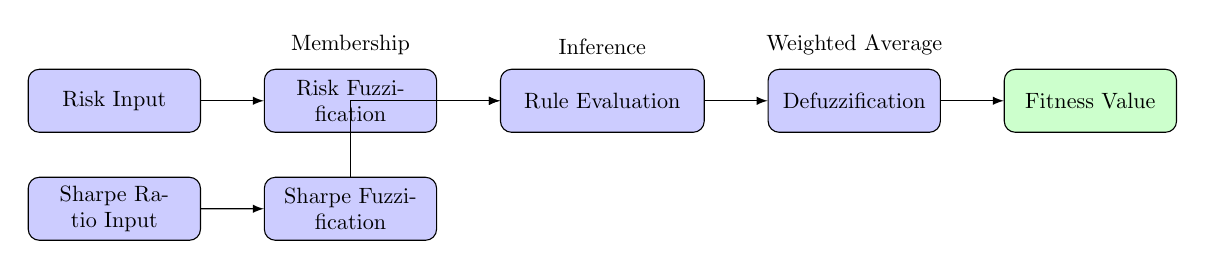
\begin{tikzpicture}[
        scale=0.8, transform shape,
        block/.style={rectangle, draw, fill=blue!20, 
                     text width=2.5cm, text centered, rounded corners, minimum height=1cm},
        line/.style={draw, -latex}
      ]
        % Input blocks
        \node [block] (risk) {Risk Input};
        \node [block, below=0.7cm of risk] (sharpe) {Sharpe Ratio Input};
        
        % Fuzzification
        \node [block, right=1cm of risk] (fuzzrisk) {Risk Fuzzification};
        \node [block, right=1cm of sharpe] (fuzzsharpe) {Sharpe Fuzzification};
        
        % Rules and inference
        \node [block, right=1cm of fuzzrisk, text width=3cm] (rules) {Rule Evaluation};
        
        % Defuzzification
        \node [block, right=1cm of rules] (defuzz) {Defuzzification};
        
        % Output
        \node [block, right=1cm of defuzz, fill=green!20] (output) {Fitness Value};
        
        % Lines
        \draw [line] (risk) -- (fuzzrisk);
        \draw [line] (sharpe) -- (fuzzsharpe);
        \draw [line] (fuzzrisk) -- (rules);
        \draw [line] (fuzzsharpe) |- (rules);
        \draw [line] (rules) -- (defuzz);
        \draw [line] (defuzz) -- (output);
        
        % Labels
        \node [above=0.1cm of fuzzrisk] {Membership};
        \node [above=0.1cm of rules] {Inference};
        \node [above=0.1cm of defuzz] {Weighted Average};
      \end{tikzpicture}
      
      \vspace{0.5cm}
      
      % Membership function visualization
      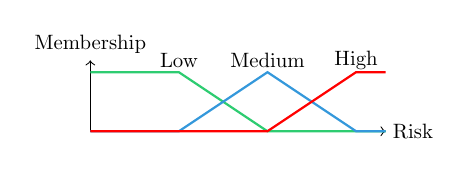
\begin{tikzpicture}[scale=0.75, transform shape]
        % Axes for Risk
        \draw[->] (0,0) -- (5,0) node[right] {Risk};
        \draw[->] (0,0) -- (0,1.2) node[above] {Membership};
        
        % Risk membership functions
        \draw[thick, fuzzygreen] (0,1) -- (1.5,1) -- (3,0) -- (5,0);
        \draw[thick, psocolor] (0,0) -- (1.5,0) -- (3,1) -- (4.5,0) -- (5,0);
        \draw[thick, red] (0,0) -- (3,0) -- (4.5,1) -- (5,1);
        
        % Labels for Risk
        \node at (1.5,1.2) {Low};
        \node at (3,1.2) {Medium};
        \node at (4.5,1.2) {High};
      \end{tikzpicture}
    \end{column}
  \end{columns}
\end{frame}

\begin{frame}{Fuzzy Logic Membership Functions}
  \centering
  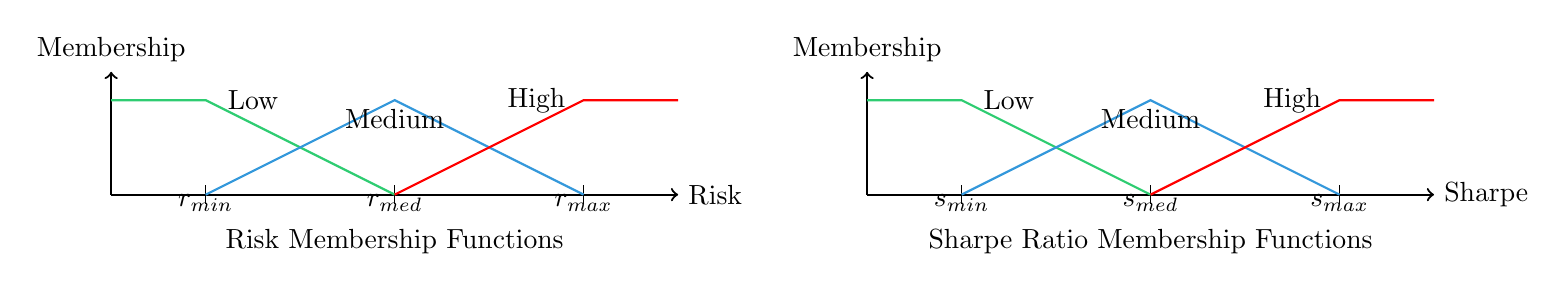
\begin{tikzpicture}[scale=1.2]
    % Risk membership functions
    \begin{scope}
      % Axes
      \draw[->,thick] (0,0) -- (6,0) node[right] {Risk};
      \draw[->,thick] (0,0) -- (0,1.3) node[above] {Membership};
      
      % Tick marks
      \foreach \x/\label in {1/r_{min}, 3/r_{med}, 5/r_{max}}
        \draw (\x,-0.1) -- (\x,0.1) node[below] {$\label$};
      
      % Functions
      \draw[thick, fuzzygreen, domain=0:3] plot (\x, {1-min(1,max(0,(\x-1)/(3-1)))});
      \draw[thick, psocolor, domain=1:5] plot (\x, {min(1, min((\x-1)/(3-1), (5-\x)/(5-3)))});
      \draw[thick, red, domain=3:6] plot (\x, {min(1,max(0,(\x-3)/(5-3)))});
      
      % Labels
      \node at (1.5,1) {Low};
      \node at (3,0.8) {Medium};
      \node at (4.5,1) {High};
      
      \node at (3,-0.5) {Risk Membership Functions};
    \end{scope}
    
    % Sharpe membership functions
    \begin{scope}[xshift=8cm]
      % Axes
      \draw[->,thick] (0,0) -- (6,0) node[right] {Sharpe};
      \draw[->,thick] (0,0) -- (0,1.3) node[above] {Membership};
      
      % Tick marks
      \foreach \x/\label in {1/s_{min}, 3/s_{med}, 5/s_{max}}
        \draw (\x,-0.1) -- (\x,0.1) node[below] {$\label$};
      
      % Functions
      \draw[thick, fuzzygreen, domain=0:3] plot (\x, {1-min(1,max(0,(\x-1)/(3-1)))});
      \draw[thick, psocolor, domain=1:5] plot (\x, {min(1, min((\x-1)/(3-1), (5-\x)/(5-3)))});
      \draw[thick, red, domain=3:6] plot (\x, {min(1,max(0,(\x-3)/(5-3)))});
      
      % Labels
      \node at (1.5,1) {Low};
      \node at (3,0.8) {Medium};
      \node at (4.5,1) {High};
      
      \node at (3,-0.5) {Sharpe Ratio Membership Functions};
    \end{scope}
  \end{tikzpicture}
\end{frame}

\begin{frame}{Fuzzy Rule Matrix}
  \centering
  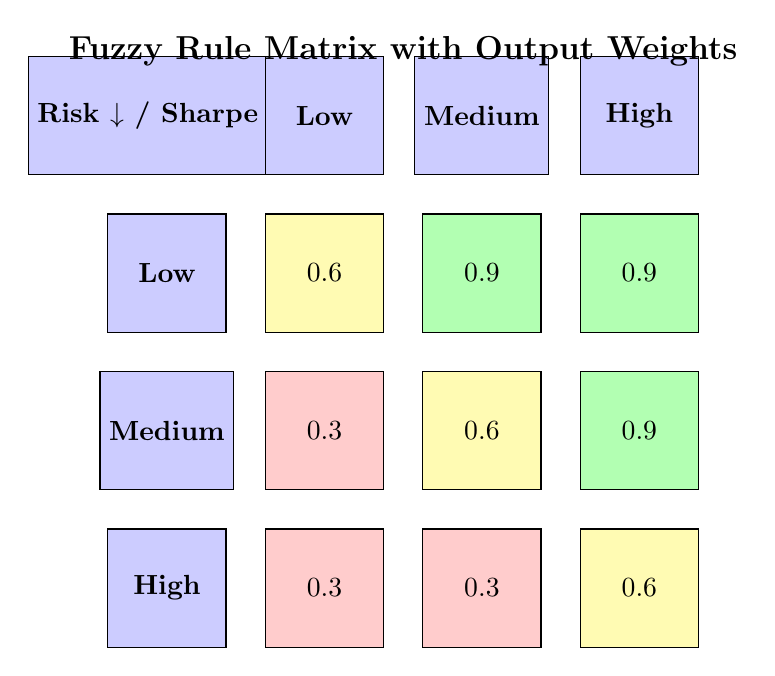
\begin{tikzpicture}[
    cell/.style={rectangle, draw, minimum size=1.5cm, text centered},
    header/.style={cell, fill=blue!20, font=\bfseries},
    value/.style={cell},
    high/.style={value, fill=green!30},
    medium/.style={value, fill=yellow!30},
    low/.style={value, fill=red!20}
  ]
    % Headers
    \node[header] at (0,0) {Risk $\downarrow$ / Sharpe $\rightarrow$};
    \node[header] at (2,0) {Low};
    \node[header] at (4,0) {Medium};
    \node[header] at (6,0) {High};
    
    \node[header] at (0,-2) {Low};
    \node[header] at (0,-4) {Medium};
    \node[header] at (0,-6) {High};
    
    % Values
    \node[medium] at (2,-2) {0.6};
    \node[high] at (4,-2) {0.9};
    \node[high] at (6,-2) {0.9};
    
    \node[low] at (2,-4) {0.3};
    \node[medium] at (4,-4) {0.6};
    \node[high] at (6,-4) {0.9};
    
    \node[low] at (2,-6) {0.3};
    \node[low] at (4,-6) {0.3};
    \node[medium] at (6,-6) {0.6};
    
    % Title
    \node[above=0.5cm] at (3,0) {\large \textbf{Fuzzy Rule Matrix with Output Weights}};
  \end{tikzpicture}
\end{frame}

\begin{frame}{Portfolio Optimization Problem Formulation}
  \begin{tcolorbox}[
    enhanced,
    colback=blue!5,
    colframe=blue!70,
    arc=2mm,
    title=Objective Function,
    fonttitle=\bfseries\large,
    boxrule=0.5mm
  ]
    Maximize the portfolio fitness derived from fuzzy inference system:
    \begin{equation}
      \max_{w} F(w) = \text{Fuzzy}(Risk(w), Sharpe(w))
    \end{equation}
    
    Where:
    \begin{align}
      Risk(w) &= \sqrt{w^T \Sigma w} \\
      Sharpe(w) &= \frac{w^T \mu - r_f}{Risk(w)}
    \end{align}
    
    $\mu$ = expected returns vector, $\Sigma$ = covariance matrix, $r_f$ = risk-free rate
  \end{tcolorbox}
  
  \vspace{0.3cm}
  
  \begin{tcolorbox}[
    enhanced,
    colback=blue!5,
    colframe=blue!70,
    arc=2mm,
    title=Constraints,
    fonttitle=\bfseries\large,
    boxrule=0.5mm
  ]
    \begin{align}
      \sum_{i=1}^{n} w_i &= 1 \quad \text{(Budget constraint)} \\
      0 \leq w_i &\leq 0.3 \quad \forall i \quad \text{(Maximum weight constraint)} \\
      \sum_{i \in S_j} w_i &\leq 0.5 \quad \forall j \quad \text{(Sector weight constraint)} \\
      \text{Max Drawdown}(w) &\leq 0.3 \quad \text{(Maximum drawdown constraint)}
    \end{align}
    
    Where $S_j$ represents the set of assets belonging to sector $j$
  \end{tcolorbox}
\end{frame}

% Section: Optimization Algorithms
\section{Optimization Algorithms}

\begin{frame}{Genetic Algorithm (GA)}
  \begin{columns}
    \begin{column}{0.55\textwidth}
      \begin{tcolorbox}[
        enhanced,
        colback=blue!5,
        colframe=blue!70,
        arc=2mm,
        title=GA Components,
        fonttitle=\bfseries\large,
        boxrule=0.5mm
      ]
        \begin{itemize}
          \item Initial population: Random weight vectors
          \item Fitness evaluation: Fuzzy-based fitness
          \item Selection: Tournament selection (size = 5)
          \item Crossover: Arithmetic crossover (alpha = random)
          \item Mutation: Random weight adjustment
          \item Elite preservation: Best 10\% solutions preserved
        \end{itemize}
      \end{tcolorbox}
      
      \vspace{0.3cm}
      
      \begin{tcolorbox}[
        enhanced,
        colback=green!5,
        colframe=green!70,
        arc=2mm,
        title=Implementation Parameters,
        fonttitle=\bfseries\large,
        boxrule=0.5mm
      ]
        \begin{itemize}
          \item Population size: 100
          \item Generations: 100
          \item Mutation rate: 0.1
          \item Crossover rate: 0.8
          \item Elite ratio: 0.1
        \end{itemize}
      \end{tcolorbox}
    \end{column}
    \begin{column}{0.45\textwidth}
      % GA flowchart will be drawn using TikZ - moved to next frame
    \end{column}
  \end{columns}
\end{frame}

\begin{frame}{Genetic Algorithm (GA) Flowchart}
  \centering
  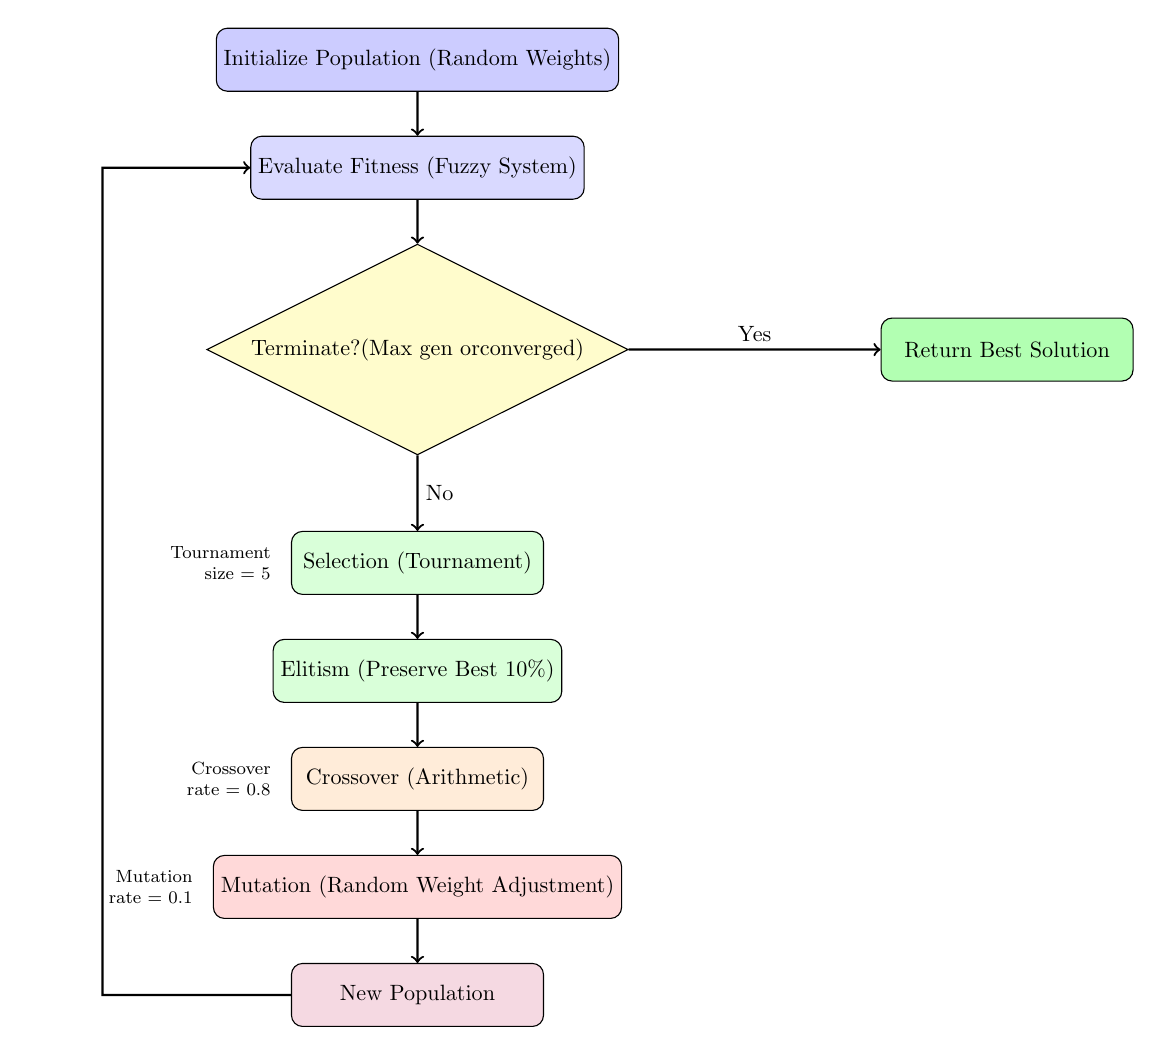
\begin{tikzpicture}[
    scale=0.8, transform shape,
    block/.style={rectangle, draw, rounded corners, minimum width=4cm, minimum height=1cm, text centered},
    decision/.style={diamond, draw, aspect=2, text centered, minimum width=3cm, minimum height=1.5cm},
    arrow/.style={thick, ->}
  ]
    % Nodes
    \node[block, fill=blue!20] (init) {Initialize Population (Random Weights)};
    \node[block, fill=blue!15, below=0.7cm of init] (eval) {Evaluate Fitness (Fuzzy System)};
    \node[decision, fill=yellow!20, below=0.7cm of eval] (term) {Terminate?\\(Max gen or\\converged)};
    \node[block, fill=green!15, below=1.2cm of term] (select) {Selection (Tournament)};
    \node[block, fill=green!15, below=0.7cm of select] (elitism) {Elitism (Preserve Best 10\%)};
    \node[block, fill=orange!15, below=0.7cm of elitism] (cross) {Crossover (Arithmetic)};
    \node[block, fill=red!15, below=0.7cm of cross] (mutate) {Mutation (Random Weight Adjustment)};
    \node[block, fill=purple!15, below=0.7cm of mutate] (new_pop) {New Population};
    \node[block, fill=green!30, right=4cm of term] (best) {Return Best Solution};
    
    % Arrows
    \draw[arrow] (init) -- (eval);
    \draw[arrow] (eval) -- (term);
    \draw[arrow] (term) -- node[right] {No} (select);
    \draw[arrow] (term) -- node[above] {Yes} (best);
    \draw[arrow] (select) -- (elitism);
    \draw[arrow] (elitism) -- (cross);
    \draw[arrow] (cross) -- (mutate);
    \draw[arrow] (mutate) -- (new_pop);
    \draw[arrow] (new_pop) -- ++(-5,0) |- (eval);
    
    % Annotations
    \node[left=0.2cm of select, text width=2.5cm, align=right, font=\footnotesize] {Tournament\\size = 5};
    \node[left=0.2cm of cross, text width=2.5cm, align=right, font=\footnotesize] {Crossover\\rate = 0.8};
    \node[left=0.2cm of mutate, text width=2.5cm, align=right, font=\footnotesize] {Mutation\\rate = 0.1};
  \end{tikzpicture}
\end{frame}

\begin{frame}{Standard Particle Swarm Optimization (PSO)}
  \begin{columns}
    \begin{column}{0.55\textwidth}
      \begin{tcolorbox}[
        enhanced,
        colback=blue!5,
        colframe=blue!70,
        arc=2mm,
        title=PSO Components,
        fonttitle=\bfseries\large,
        boxrule=0.5mm
      ]
        \begin{itemize}
          \item Swarm: Collection of particles (potential portfolios)
          \item Particle position: Portfolio weights
          \item Particle velocity: Search direction and step size
          \item Personal best: Best position found by each particle
          \item Global best: Best position found by the entire swarm
          \item Movement: Balance between exploration and exploitation
        \end{itemize}
      \end{tcolorbox}
      
      \vspace{0.3cm}
      
      \begin{tcolorbox}[
        enhanced,
        colback=green!5,
        colframe=green!70,
        arc=2mm,
        title=Implementation Parameters,
        fonttitle=\bfseries\large,
        boxrule=0.5mm
      ]
        \begin{itemize}
          \item Number of particles: 100
          \item Iterations: 100
          \item Inertia weight ($w$): 0.7
          \item Cognitive coefficient ($c_1$): 1.5
          \item Social coefficient ($c_2$): 1.5
          \item Velocity clamping: 0.1
        \end{itemize}
      \end{tcolorbox}
    \end{column}
    
    \begin{column}{0.45\textwidth}
      \begin{align}
        v_i^{t+1} = w \cdot v_i^t &+ c_1 r_1 (p_i - x_i^t) \\
        &+ c_2 r_2 (g - x_i^t) \nonumber \\
        x_i^{t+1} &= x_i^t + v_i^{t+1}
      \end{align}
      
      \vspace{0.3cm}
      Where:
      \begin{itemize}
        \item $v_i^t$: Velocity of particle $i$ at time $t$
        \item $x_i^t$: Position (portfolio weights) of particle $i$
        \item $p_i$: Personal best position of particle $i$
        \item $g$: Global best position (best portfolio)
        \item $r_1, r_2$: Random numbers in $[0,1]$
        \item $w$: Inertia weight (controls momentum)
        \item $c_1$: Cognitive coefficient (self-confidence)
        \item $c_2$: Social coefficient (swarm confidence)
      \end{itemize}
    \end{column}
  \end{columns}
\end{frame}

\begin{frame}{Standard PSO Algorithm Visualization}
  \centering
  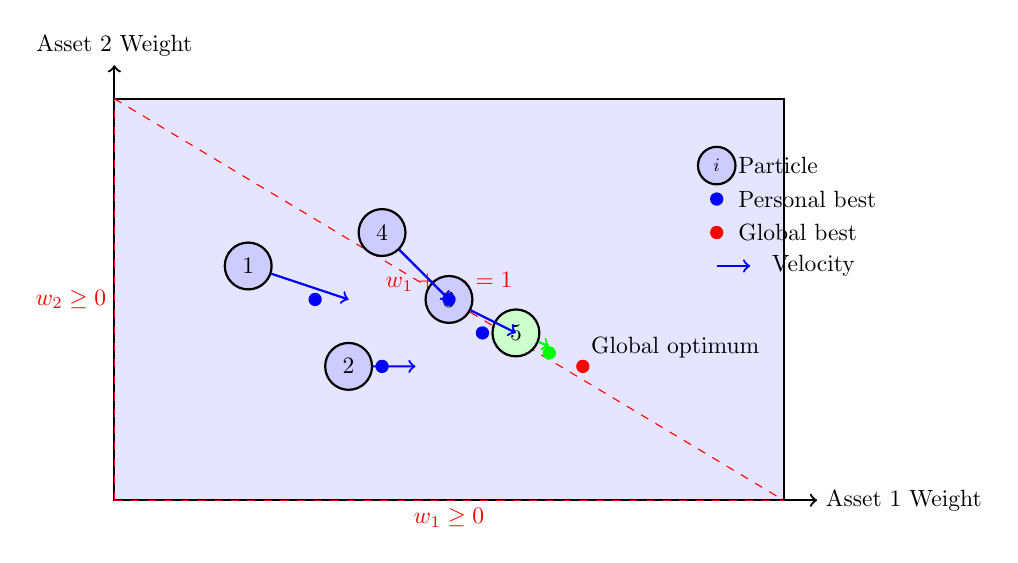
\begin{tikzpicture}[
    scale=0.85, transform shape,
    dot/.style={circle, fill, inner sep=2pt},
    particle/.style={circle, draw, thick, minimum size=0.7cm}
  ]
    % Search space background
    \fill[blue!10] (0,0) rectangle (10,6);
    \draw[thick] (0,0) rectangle (10,6);
    
    % Axes
    \draw[->, thick] (0,0) -- (10.5,0) node[right] {Asset 1 Weight};
    \draw[->, thick] (0,0) -- (0,6.5) node[above] {Asset 2 Weight};
    
    % Constraint lines
    \draw[dashed, red] (0,0) -- (10,0) node[midway, below] {$w_1 \geq 0$};
    \draw[dashed, red] (0,0) -- (0,6) node[midway, left] {$w_2 \geq 0$};
    \draw[dashed, red] (0,6) -- (10,0) node[midway, above] {$w_1 + w_2 = 1$};
    
    % Global optimum
    \node[dot, color=red] (opt) at (7,2) {};
    \node[above right] at (opt) {Global optimum};
    
    % Particles
    \node[particle, fill=blue!20] (p1) at (2,3.5) {1};
    \node[particle, fill=blue!20] (p2) at (3.5,2) {2};
    \node[particle, fill=blue!20] (p3) at (5,3) {3};
    \node[particle, fill=blue!20] (p4) at (4,4) {4};
    \node[particle, fill=green!20] (p5) at (6,2.5) {5};
    
    % Velocity vectors
    \draw[->, thick, blue] (p1) -- ++(1.5,-0.5);
    \draw[->, thick, blue] (p2) -- ++(1,0);
    \draw[->, thick, blue] (p3) -- ++(1,-0.5);
    \draw[->, thick, blue] (p4) -- ++(1,-1);
    \draw[->, thick, green] (p5) -- ++(0.5,-0.2);
    
    % Personal bests
    \node[dot, color=blue] at (3,3) {};
    \node[dot, color=blue] at (4,2) {};
    \node[dot, color=blue] at (5.5,2.5) {};
    \node[dot, color=blue] at (5,3) {};
    \node[dot, color=green] at (6.5,2.2) {};
    
    % Legend
    \node[particle, fill=blue!20, scale=0.8] at (9,5) {$i$};
    \node[right=0.2cm of {(9,5)}] {Particle};
    \node[dot, color=blue] at (9,4.5) {};
    \node[right=0.2cm of {(9,4.5)}] {Personal best};
    \node[dot, color=red] at (9,4) {};
    \node[right=0.2cm of {(9,4)}] {Global best};
    \draw[->, thick, blue] (9,3.5) -- ++(0.5,0);
    \node[right=0.7cm of {(9,3.5)}] {Velocity};
  \end{tikzpicture}
  
  \vspace{0.3cm}
  \small{Each particle represents a portfolio allocation that moves through the solution space guided by its own experience and the swarm's collective knowledge.}
\end{frame}

\begin{frame}{Adaptive PSO}
  \begin{columns}
    \begin{column}{0.55\textwidth}
      \begin{tcolorbox}[
        enhanced,
        colback=blue!5,
        colframe=blue!70,
        arc=2mm,
        title=Adaptive Parameters,
        fonttitle=\bfseries\large,
        boxrule=0.5mm
      ]
        \begin{itemize}
          \item Dynamically adjusts parameters during optimization
          \item Inertia weight ($w$): Decreases linearly from 0.9 to 0.4
          \item Cognitive parameter ($c_1$): Decreases from 2.5 to 1.5
          \item Social parameter ($c_2$): Increases from 1.5 to 2.5
          \item Velocity clamping based on swarm diversity
        \end{itemize}
      \end{tcolorbox}
      
      \vspace{0.3cm}
      
      \begin{tcolorbox}[
        enhanced,
        colback=green!5,
        colframe=green!70,
        arc=2mm,
        title=Adaptation Formulas,
        fonttitle=\bfseries\large,
        boxrule=0.5mm
      ]
        \begin{align}
          w &= w_{max} - \frac{iter}{max\_iter} \cdot (w_{max} - w_{min}) \\
          c_1 &= c_{1\_init} - \frac{iter}{max\_iter} \cdot (c_{1\_init} - c_{1\_final}) \\
          c_2 &= c_{2\_init} + \frac{iter}{max\_iter} \cdot (c_{2\_final} - c_{2\_init})
        \end{align}
      \end{tcolorbox}
    \end{column}
    
    \begin{column}{0.45\textwidth}
      % Graph showing parameter changes
      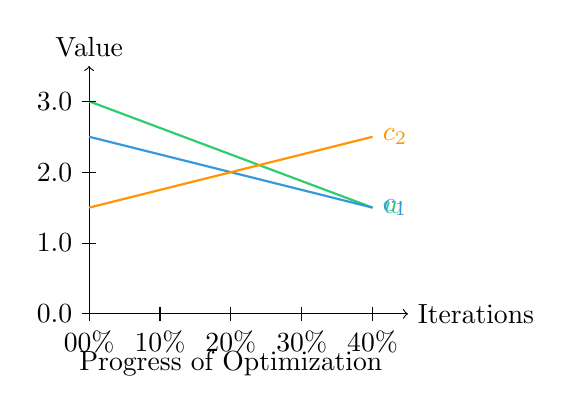
\begin{tikzpicture}[scale=0.9]
        \draw[->] (0,0) -- (4.5,0) node[right] {Iterations};
        \draw[->] (0,0) -- (0,3.5) node[above] {Value};
        
        % Parameter curves
        \draw[thick, fuzzygreen] (0,3) -- (4,1.5) node[right] {$w$};
        \draw[thick, psocolor] (0,2.5) -- (4,1.5) node[right] {$c_1$};
        \draw[thick, adaptivecolor] (0,1.5) -- (4,2.5) node[right] {$c_2$};
        
        % Axes ticks
        \foreach \x in {0,1,2,3,4}
          \draw (\x,0.1) -- (\x,-0.1) node[below] {\x0\%};
        \foreach \y in {0,1,2,3}
          \draw (0.1,\y) -- (-0.1,\y) node[left] {\y.0};
          
        \node at (2,-0.7) {Progress of Optimization};
      \end{tikzpicture}
      
      \vspace{0.5cm}
      
      \begin{tcolorbox}[
        enhanced,
        colback=yellow!5,
        colframe=yellow!70,
        arc=2mm,
        title=Benefits,
        fonttitle=\bfseries\large,
        boxrule=0.5mm
      ]
        \begin{itemize}
          \item Early emphasis on exploration (high $w$, high $c_1$)
          \item Later emphasis on exploitation (low $w$, high $c_2$)
          \item Prevents premature convergence
          \item Adapts to the optimization landscape
          \item No parameter tuning needed
        \end{itemize}
      \end{tcolorbox}
    \end{column}
  \end{columns}
\end{frame}

\begin{frame}{Parallel PSO Architecture}
  \centering
  \begin{tikzpicture}[
    scale=0.75, transform shape,
    block/.style={rectangle, draw, rounded corners, minimum width=4cm, minimum height=1cm, text centered},
    decision/.style={diamond, draw, aspect=2, text centered, minimum width=3cm, minimum height=1.5cm},
    arrow/.style={thick, ->}
  ]
    % Main nodes
    \node[block, fill=blue!20] (init) {Initialize Particles};
    \node[block, fill=blue!15, below=0.7cm of init] (split) {Split Particles Among Processes};
    
    % Worker nodes (side by side)
    \node[block, fill=green!15, below=1.5cm of split, xshift=-4cm] (w1) {Worker Process 1};
    \node[block, fill=green!15, below=1.5cm of split] (w2) {Worker Process 2};
    \node[block, fill=green!15, below=1.5cm of split, xshift=4cm] (w3) {Worker Process N};
    
    % Sync and evaluate
    \node[block, fill=orange!15, below=2.5cm of split] (sync) {Synchronize Results};
    \node[block, fill=yellow!15, below=0.7cm of sync] (update) {Update Global Best};
    \node[decision, fill=yellow!20, below=0.7cm of update] (term) {Terminate?};
    \node[block, fill=red!30, below right=1cm and 2cm of term] (best) {Return Best Solution};
    
    % Connect the dots
    \draw[arrow] (init) -- (split);
    \draw[arrow] (split) -- (w1);
    \draw[arrow] (split) -- (w2);
    \draw[arrow] (split) -- (w3);
    \node at (0, -2.5) {\ldots};
    
    \draw[arrow] (w1) -- ++(0, -1.5) -| (sync);
    \draw[arrow] (w2) -- (sync);
    \draw[arrow] (w3) -- ++(0, -1.5) -| (sync);
    
    \draw[arrow] (sync) -- (update);
    \draw[arrow] (update) -- (term);
    \draw[arrow] (term) -- node[above] {Yes} (best);
    \draw[arrow] (term) -- node[left] {No} ++(-4,0) |- (split);
    
    % Process details boxes
    \node[draw, dashed, fill=blue!5, rounded corners, fit={(w1) ($(w1)+(0,-0.7)$)}, inner sep=0.2cm] (p1) {};
    \node[draw, dashed, fill=blue!5, rounded corners, fit={(w2) ($(w2)+(0,-0.7)$)}, inner sep=0.2cm] (p2) {};
    \node[draw, dashed, fill=blue!5, rounded corners, fit={(w3) ($(w3)+(0,-0.7)$)}, inner sep=0.2cm] (p3) {};
    
    \node[below=0.1cm of w1, text width=2.5cm, align=center, font=\footnotesize] {Update Positions \& Velocities};
    \node[below=0.1cm of w2, text width=2.5cm, align=center, font=\footnotesize] {Update Positions \& Velocities};
    \node[below=0.1cm of w3, text width=2.5cm, align=center, font=\footnotesize] {Update Positions \& Velocities};
    
    % Title
    \node[above=0.3cm of init, font=\Large\bfseries] {Parallel PSO Architecture};
  \end{tikzpicture}
\end{frame}

\begin{frame}{Island Model PSO}
  \centering
  \begin{tikzpicture}[
    scale=0.7, transform shape,
    island/.style={ellipse, draw, fill=blue!10, minimum width=3.5cm, minimum height=2.2cm},
    particle/.style={circle, draw, fill=blue!20, minimum size=0.5cm},
    migration/.style={thick, ->, >=stealth, dashed, blue},
    particle_label/.style={font=\tiny}
  ]
    % Islands
    \node[island] (i1) at (0,0) {Island 1};
    \node[island] (i2) at (6,0) {Island 2};
    \node[island] (i3) at (6,-4) {Island 3};
    \node[island] (i4) at (0,-4) {Island 4};
    
    % Particles in each island
    \foreach \i in {1,2,3,4,5} {
      \node[particle] (p1\i) at ($(i1) + ({360/5 * \i}:1cm)$) {\i};
    }
    
    \foreach \i in {1,2,3,4,5} {
      \node[particle] (p2\i) at ($(i2) + ({360/5 * \i}:1cm)$) {\i};
    }
    
    \foreach \i in {1,2,3,4,5} {
      \node[particle] (p3\i) at ($(i3) + ({360/5 * \i}:1cm)$) {\i};
    }
    
    \foreach \i in {1,2,3,4,5} {
      \node[particle] (p4\i) at ($(i4) + ({360/5 * \i}:1cm)$) {\i};
    }
    
    % Migration paths
    \draw[migration] (i1) to [bend left=15] node[midway, above] {Migration} (i2);
    \draw[migration] (i2) to [bend left=15] node[midway, right] {Migration} (i3);
    \draw[migration] (i3) to [bend left=15] node[midway, below] {Migration} (i4);
    \draw[migration] (i4) to [bend left=15] node[midway, left] {Migration} (i1);
    
    % Process flows within each island
    \node[draw, rounded corners, fill=yellow!20, font=\footnotesize] at ($(i1) + (0,-1.5)$) {Local PSO Process};
    \node[draw, rounded corners, fill=yellow!20, font=\footnotesize] at ($(i2) + (0,-1.5)$) {Local PSO Process};
    \node[draw, rounded corners, fill=yellow!20, font=\footnotesize] at ($(i3) + (0,-1.5)$) {Local PSO Process};
    \node[draw, rounded corners, fill=yellow!20, font=\footnotesize] at ($(i4) + (0,-1.5)$) {Local PSO Process};
    
    % Title and legend
    \node[font=\Large\bfseries] at (3,-6) {Island Model PSO Architecture};
    
    \node[draw, fill=blue!10, rounded corners] at (10,-1) {Legend:};
    \node[particle] at (10,-1.5) {};
    \node[right=0.2cm of {(10,-1.5)}] {Particle};
    \node[island, minimum width=2cm, minimum height=1cm] at (11,-2.5) {Island};
    \draw[migration] (9.5,-3.2) -- ++(1.5,0);
    \node[right=1.8cm of {(9.5,-3.2)}] {Migration};
  \end{tikzpicture}
\end{frame}

% Section: Results
\section{Results}

\begin{frame}{Speed vs. Quality Trade-off}
  \centering
  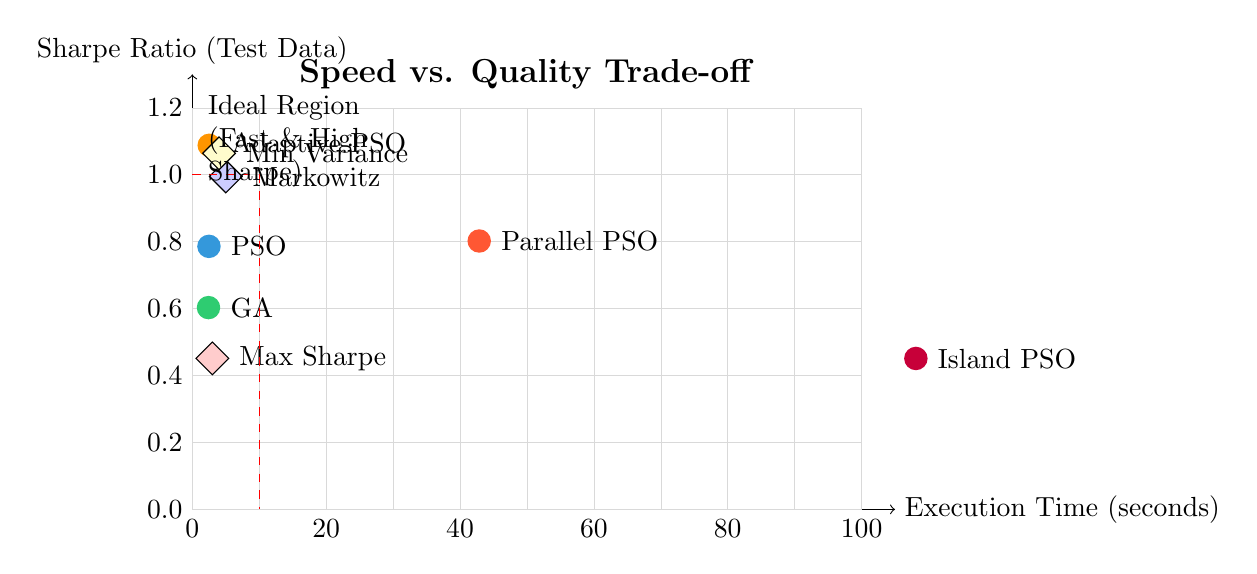
\begin{tikzpicture}[scale=0.85]
    % Axes
    \draw[->] (0,0) -- (10.5,0) node[right] {Execution Time (seconds)};
    \draw[->] (0,0) -- (0,6.5) node[above] {Sharpe Ratio (Test Data)};
    
    % Grid
    \draw[gray!30, very thin] (0,0) grid (10,6);
    
    % Data points
    \node[circle, fill=fuzzygreen, inner sep=3pt, label=right:GA] (ga) at (2.42*0.1,0.603*5) {};
    \node[circle, fill=psocolor, inner sep=3pt, label=right:PSO] (pso) at (2.49*0.1,0.786*5) {};
    \node[circle, fill=adaptivecolor, inner sep=3pt, label=right:Adaptive PSO] (adaptive) at (2.53*0.1,1.088*5) {};
    \node[circle, fill=parallelcolor, inner sep=3pt, label=right:Parallel PSO] (parallel) at (4.287,0.802*5) {};
    \node[circle, fill=islandcolor, inner sep=3pt, label=right:Island PSO] (island) at (10.811,0.451*5) {};
    
    % Traditional methods for comparison
    \node[diamond, draw, fill=blue!20, inner sep=3pt, label=right:Markowitz] (markowitz) at (0.5,0.995*5) {};
    \node[diamond, draw, fill=yellow!20, inner sep=3pt, label=right:Min Variance] (minvar) at (0.4,1.064*5) {};
    \node[diamond, draw, fill=red!20, inner sep=3pt, label=right:Max Sharpe] (maxsharpe) at (0.3,0.451*5) {};
    
    % Ideal region
    \draw[dashed, red] (0,5) -- (1,5);
    \draw[dashed, red] (1,5) -- (1,0);
    \node[text width=3cm] at (2,5.5) {Ideal Region\\(Fast \& High Sharpe)};
    
    % Labels
    \foreach \x/\label in {0/0, 2/20, 4/40, 6/60, 8/80, 10/100}
      \node[below] at (\x,0) {\label};
    
    \foreach \y/\label in {0/0.0, 1/0.2, 2/0.4, 3/0.6, 4/0.8, 5/1.0, 6/1.2}
      \node[left] at (0,\y) {\label};
    
    % Title
    \node at (5,6.5) {\large \textbf{Speed vs. Quality Trade-off}};
  \end{tikzpicture}
\end{frame}

\begin{frame}{Analysis of Speed vs. Quality Trade-off}
  \begin{tcolorbox}[
    enhanced,
    colback=blue!5,
    colframe=blue!70,
    arc=2mm,
    title=Analysis,
    fonttitle=\bfseries\large,
    boxrule=0.5mm
  ]
    \begin{itemize}
      \item Adaptive PSO offers best balance of execution speed and performance quality
      \item Parallel implementations introduce significant overhead without performance gain
      \item Traditional methods (Markowitz, Min Variance) are fast but require different objective
      \item Island Model PSO provides no advantage in this portfolio size (30 assets)
    \end{itemize}
  \end{tcolorbox}
  
  \begin{tcolorbox}[
    enhanced,
    colback=green!5,
    colframe=green!70,
    arc=2mm,
    title=Key Insights,
    fonttitle=\bfseries\large,
    boxrule=0.5mm
  ]
    \begin{itemize}
      \item Communication overhead dominates execution time in parallel implementations
      \item Adaptive parameter tuning improves solution quality without additional computational cost
      \item Traditional Max Sharpe solution performs poorly in out-of-sample testing
      \item For small to medium portfolios, sequential optimization methods are preferred
    \end{itemize}
  \end{tcolorbox}
\end{frame}

\begin{frame}{Convergence Analysis}
  \centering
  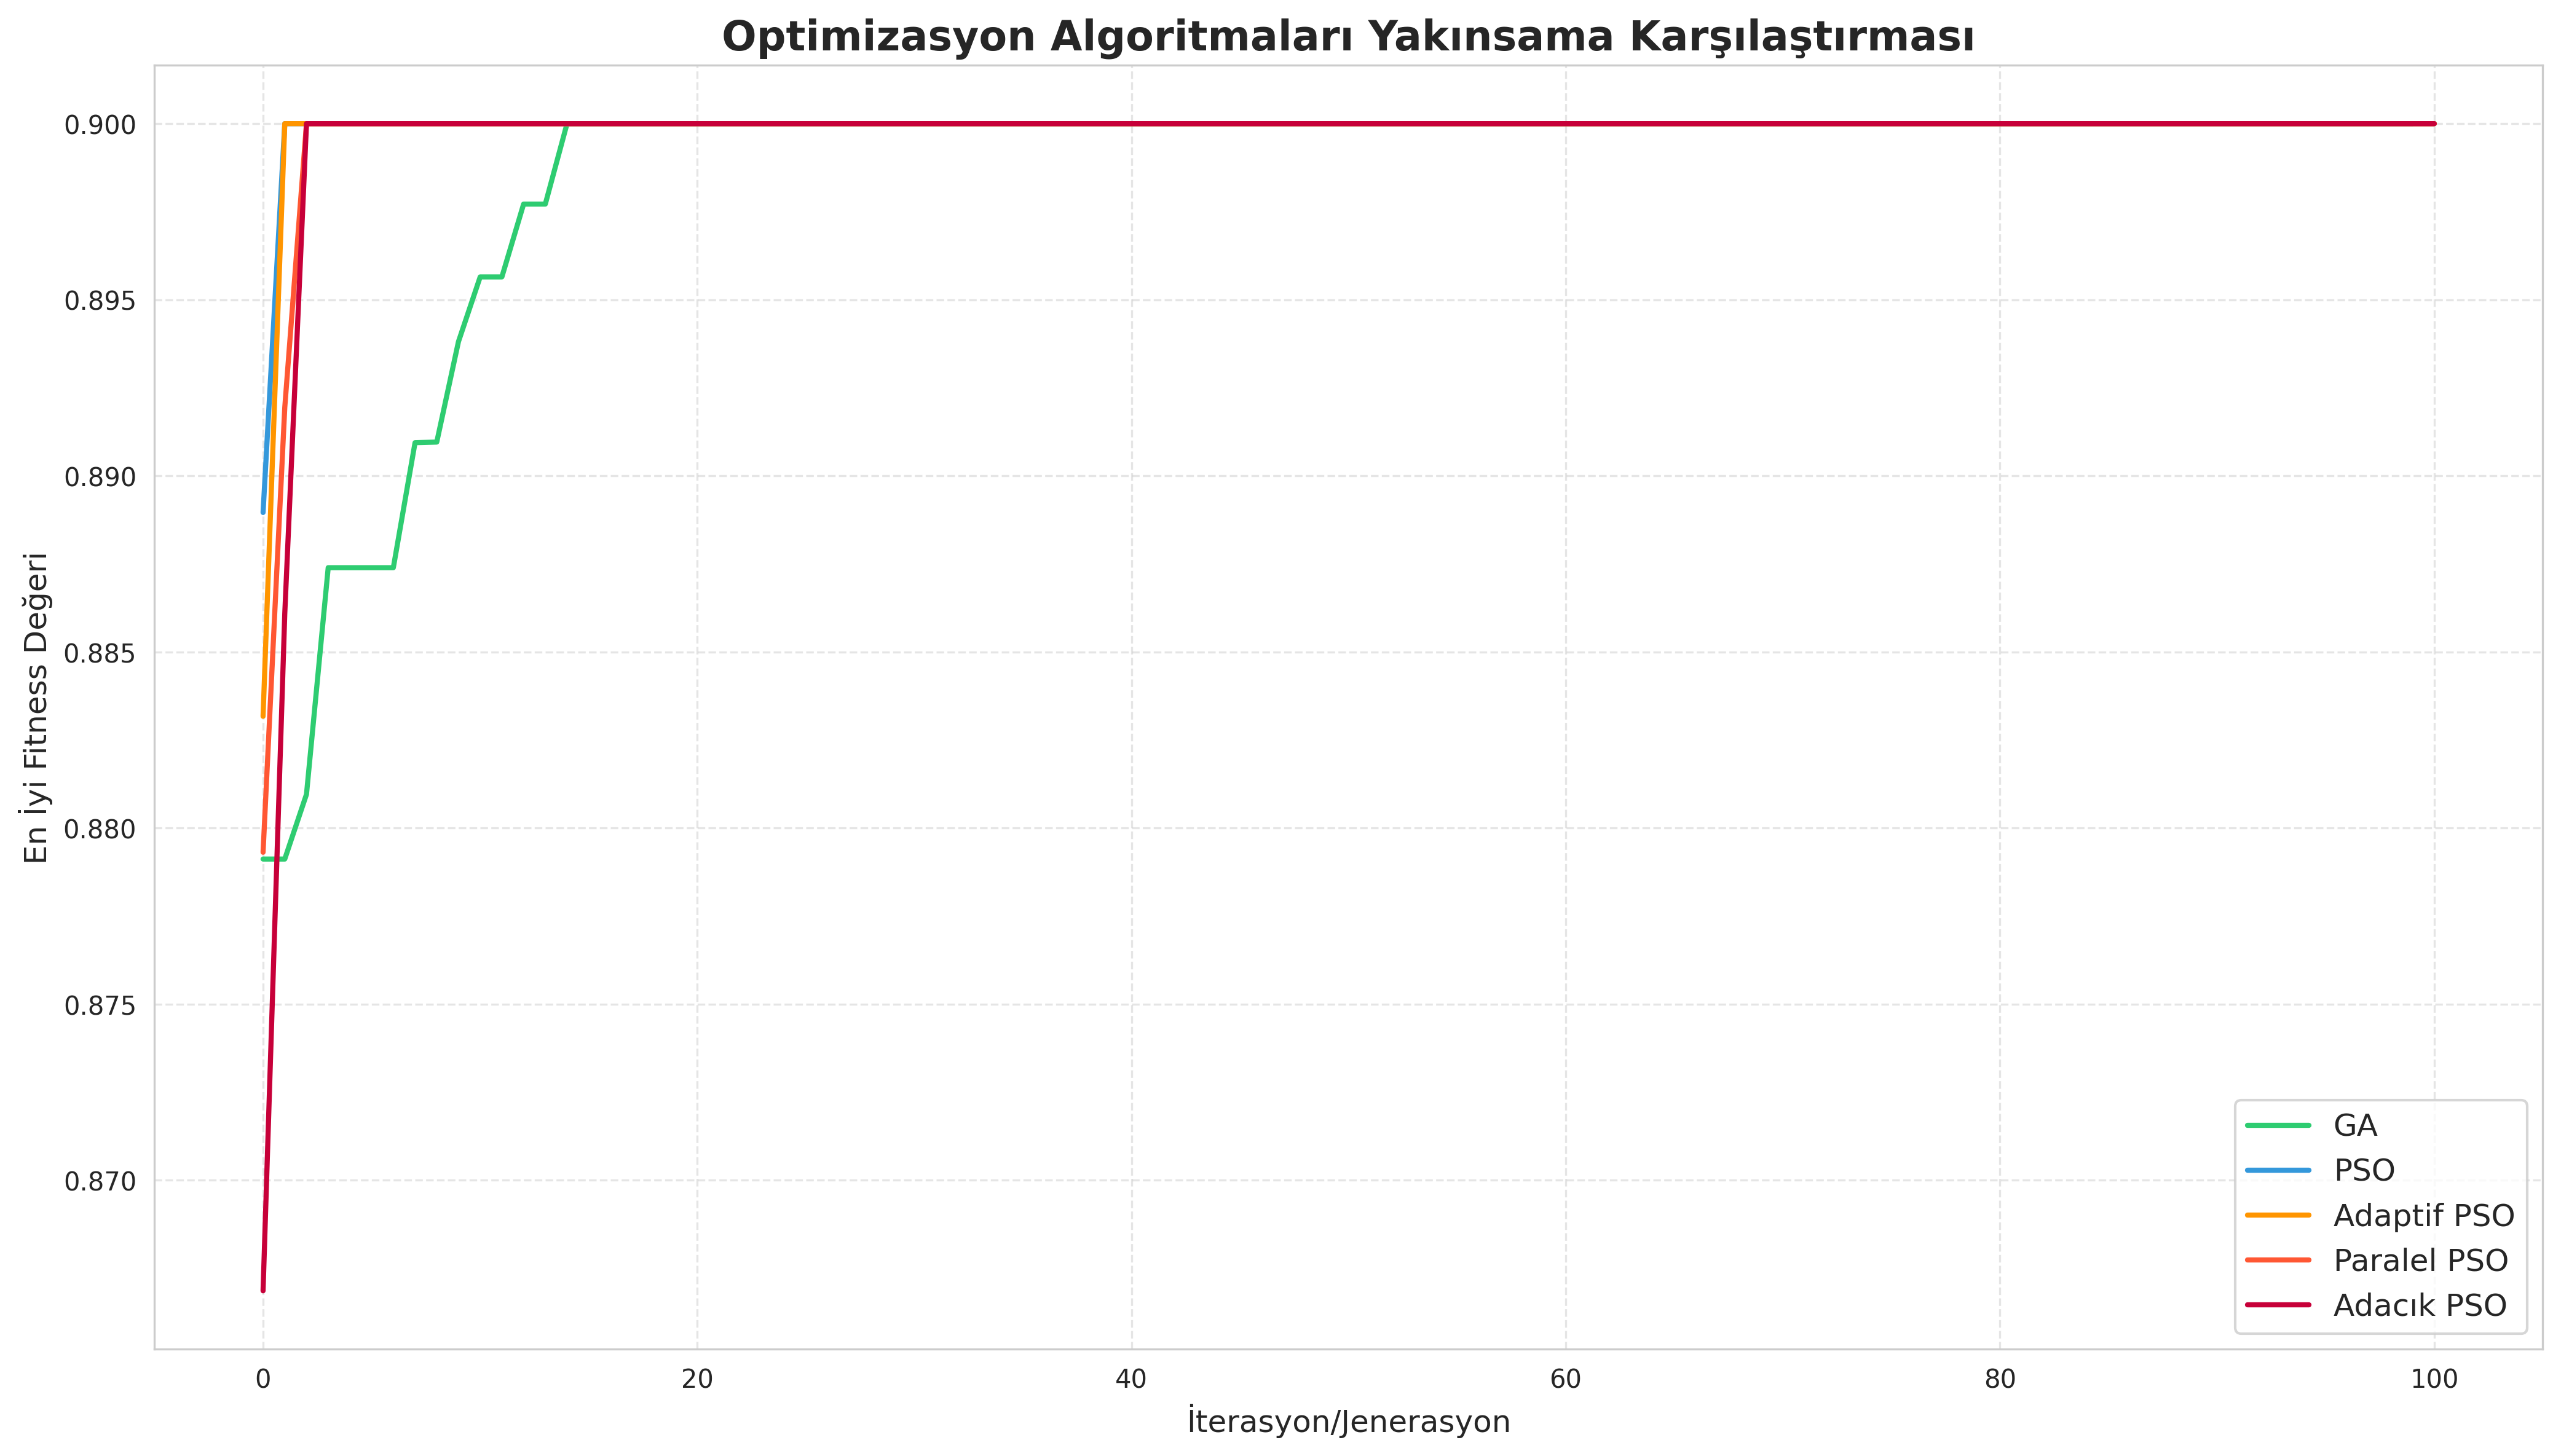
\includegraphics[width=\textwidth, height=5.5cm, keepaspectratio]{convergence_comparison.png}
  % This shows the optimization algorithms convergence comparison chart
  
  \begin{tcolorbox}[
    enhanced,
    colback=blue!5,
    colframe=blue!70,
    arc=2mm,
    title=Observations,
    fonttitle=\bfseries\large,
    boxrule=0.5mm
  ]
    \begin{itemize}
      \item All algorithms eventually reached similar fitness values (0.9)
      \item Adaptive PSO and Standard PSO showed fastest initial convergence
      \item Island Model PSO exhibited occasional jumps due to migrations
      \item GA demonstrated more gradual improvement
      \item Parallel PSO showed similar convergence pattern to Standard PSO
    \end{itemize}
  \end{tcolorbox}
\end{frame}

\begin{frame}{Portfolio Composition}
  \centering
  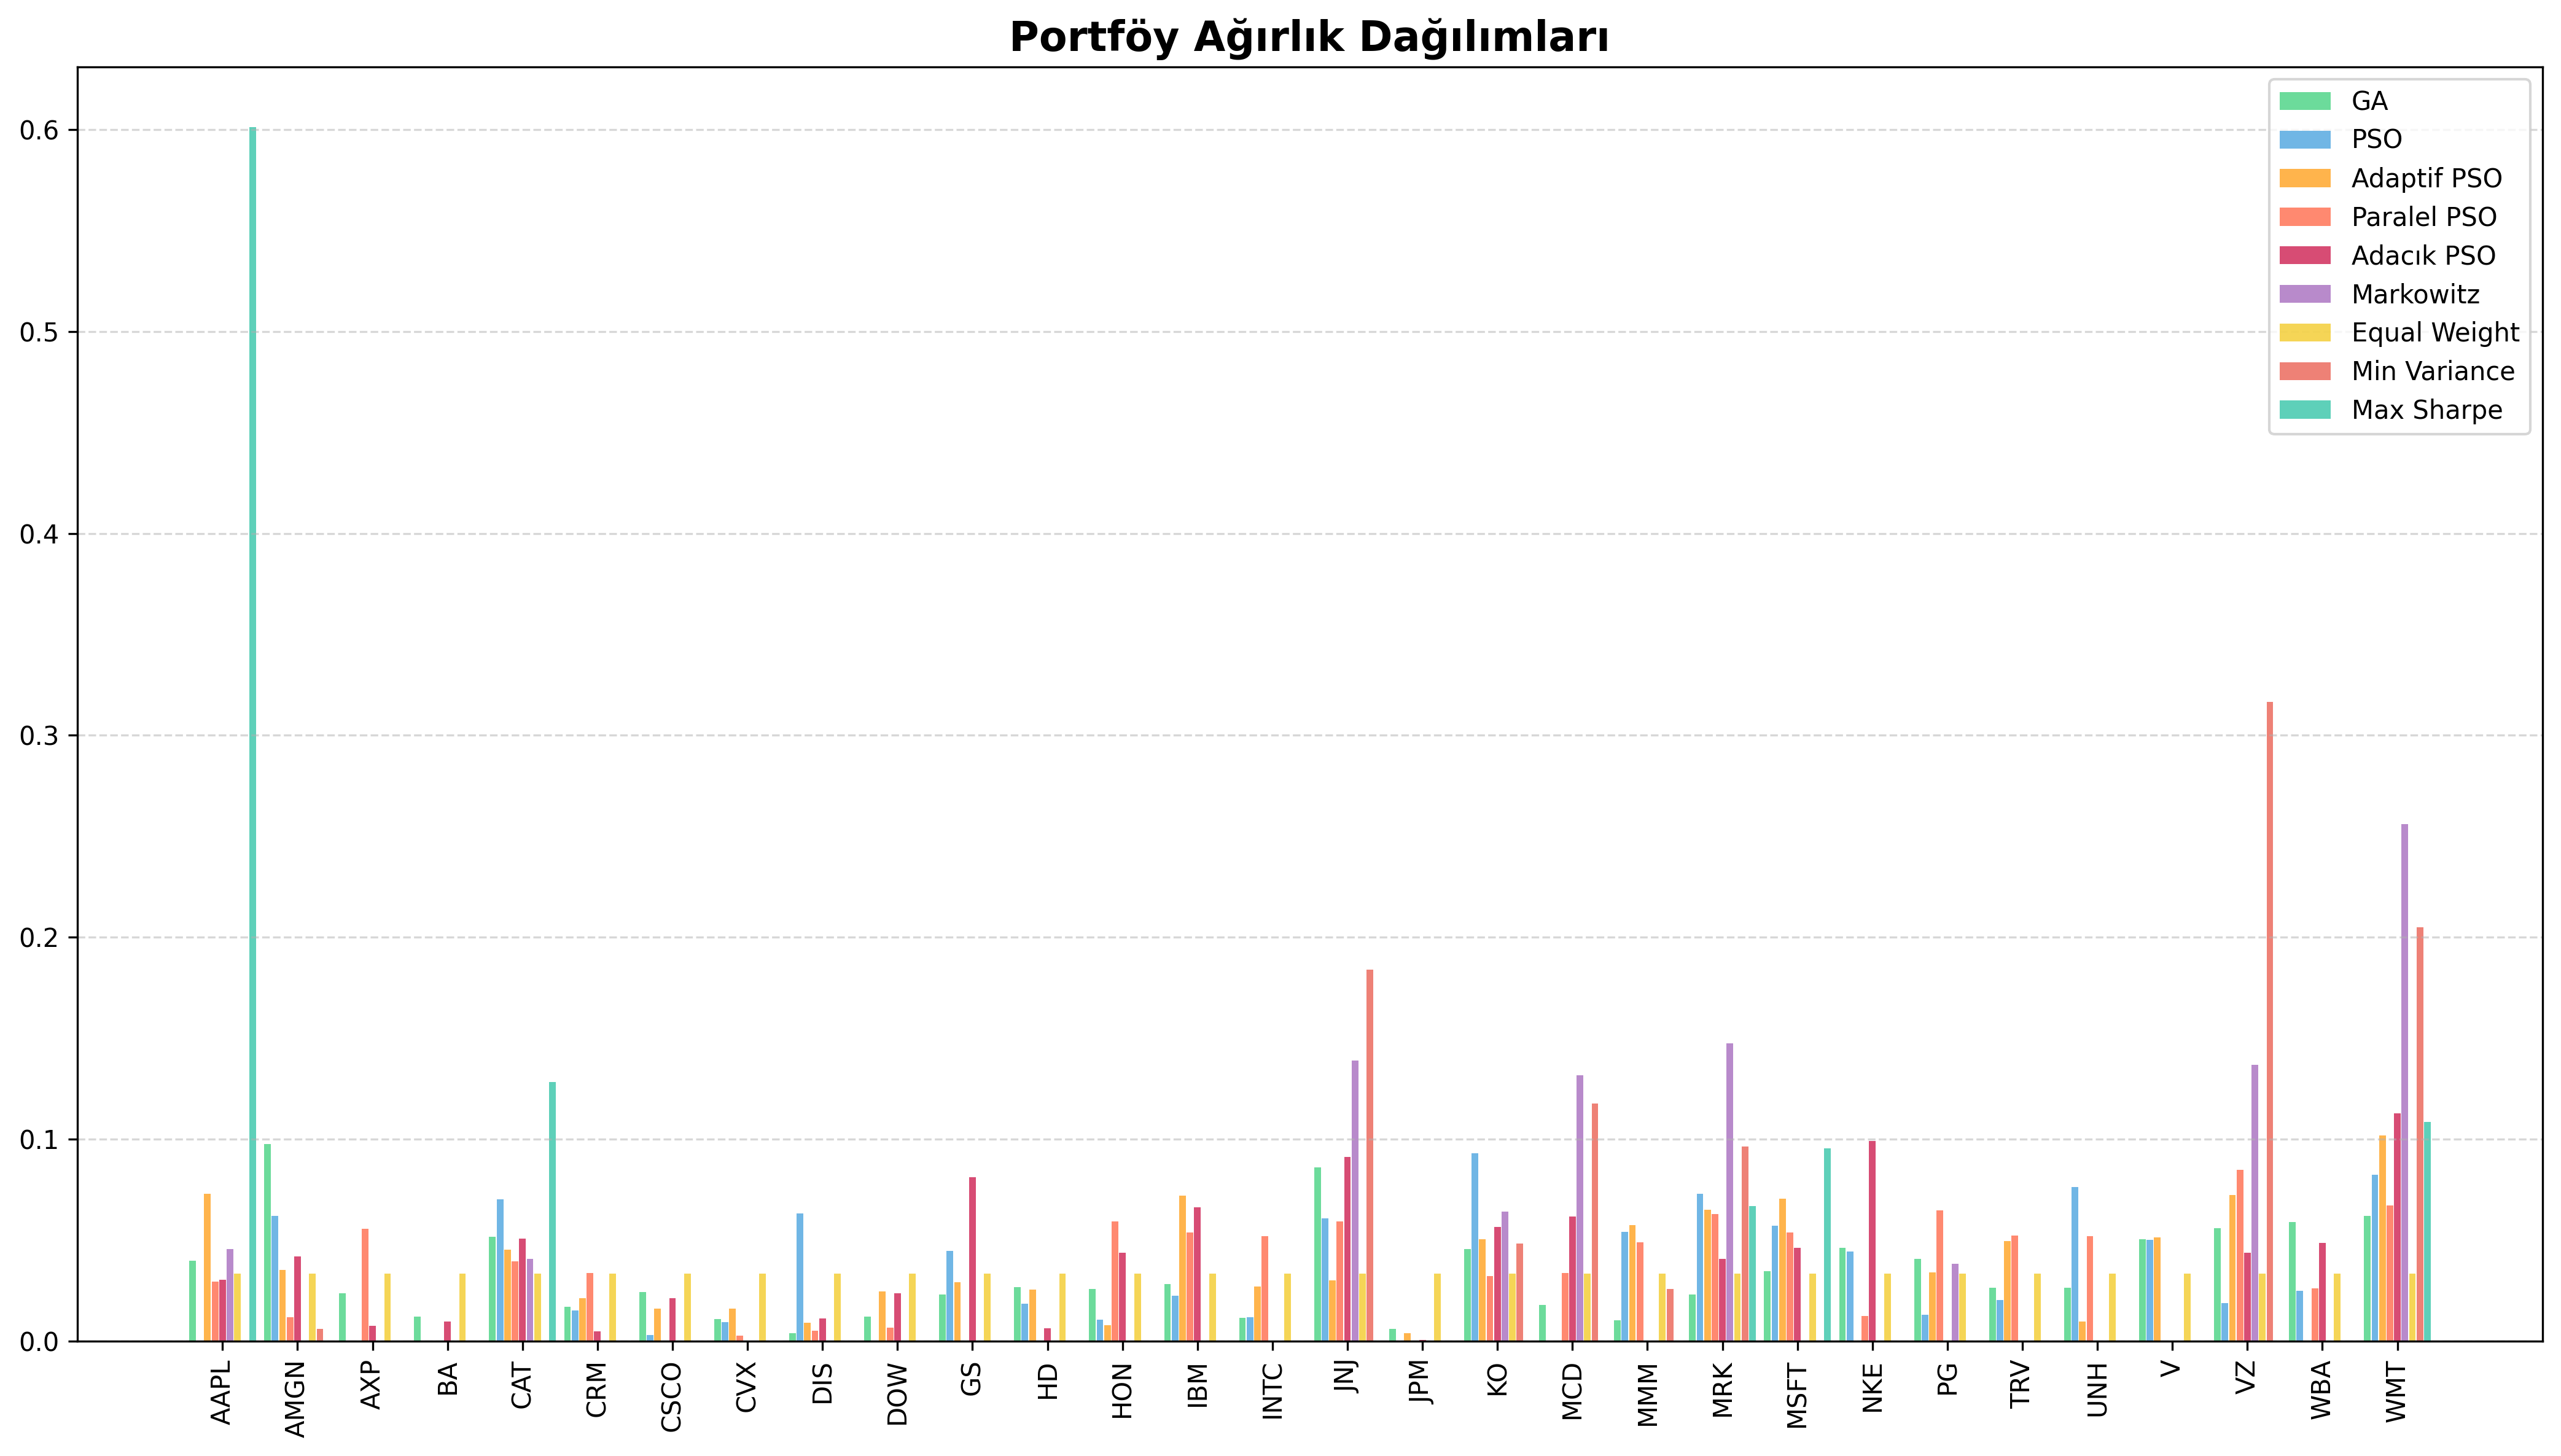
\includegraphics[width=\textwidth, height=5.5cm, keepaspectratio]{portfolio_weights_comparison.png}
  % This shows the portfolio weight distributions across different assets
  
  \begin{tcolorbox}[
    enhanced,
    colback=blue!5,
    colframe=blue!70,
    arc=2mm,
    title=Analysis of Weight Distributions,
    fonttitle=\bfseries\large,
    boxrule=0.5mm
  ]
    \begin{itemize}
      \item Significant differences in asset allocation across algorithms
      \item Adaptive PSO and Min Variance favored less volatile stocks
      \item Island Model PSO showed higher concentration in fewer assets
      \item GA and Standard PSO produced more diversified portfolios
      \item Max Sharpe solution heavily concentrated in AAPL
      \item All algorithms respected maximum weight constraint (30\%)
    \end{itemize}
  \end{tcolorbox}
\end{frame}

\begin{frame}{Performance Metrics - Test Data}
  \centering
  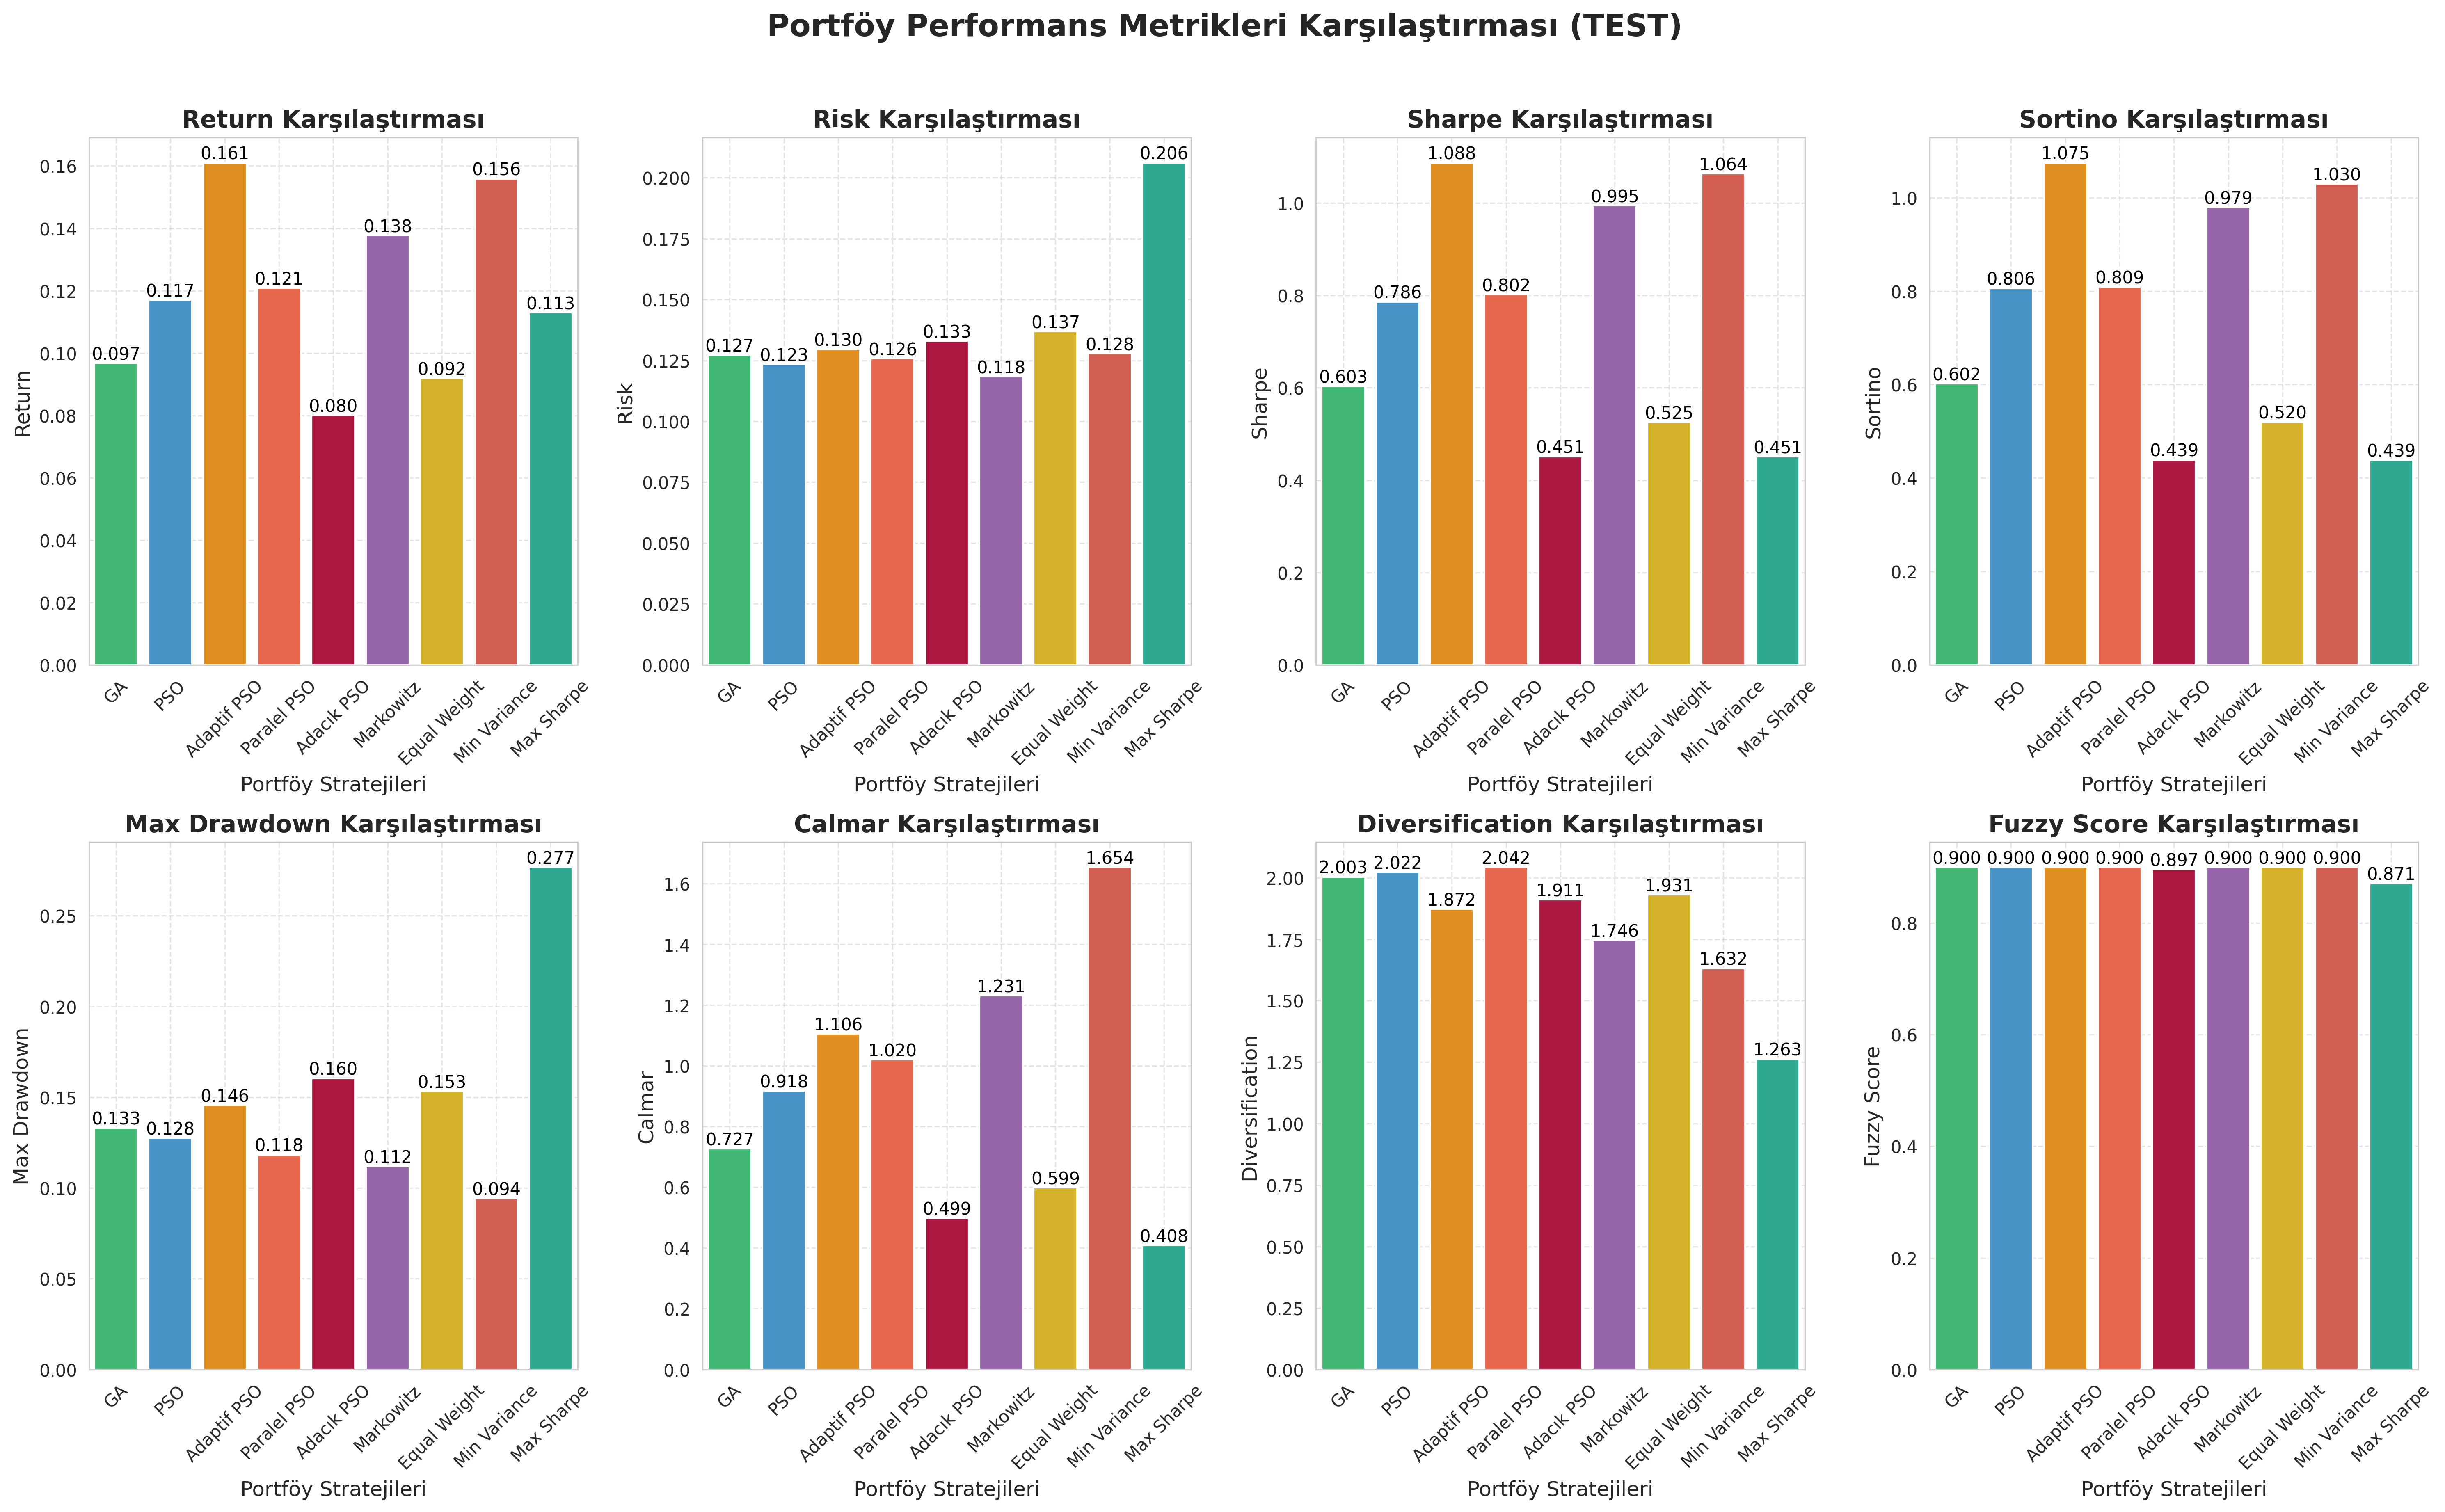
\includegraphics[width=\textwidth, height=5.5cm, keepaspectratio]{test_performance_metrics_comparison.png}
  % This shows the test performance metrics for all portfolio strategies
  
  \begin{columns}
    \begin{column}{0.48\textwidth}
      \begin{tcolorbox}[
        enhanced,
        colback=green!5,
        colframe=green!70,
        arc=2mm,
        title=Top Performers,
        fonttitle=\bfseries\large,
        boxrule=0.5mm
      ]
        \begin{itemize}
          \item Adaptive PSO: Highest Sharpe (1.088) and Sortino (1.075)
          \item Min Variance: Lowest Max Drawdown (0.094)
          \item Markowitz: Lowest Risk (0.118)
          \item Parallel PSO: Good balance of metrics
        \end{itemize}
      \end{tcolorbox}
    \end{column}
    \begin{column}{0.48\textwidth}
      \begin{tcolorbox}[
        enhanced,
        colback=red!5,
        colframe=red!70,
        arc=2mm,
        title=Surprising Results,
        fonttitle=\bfseries\large,
        boxrule=0.5mm
      ]
        \begin{itemize}
          \item Max Sharpe underperformed with highest risk (0.206)
          \item Equal Weight performed better than expected
          \item Island Model PSO showed lower Sharpe despite complex architecture
          \item All fuzzy-guided approaches received similar fuzzy scores
        \end{itemize}
      \end{tcolorbox}
    \end{column}
  \end{columns}
\end{frame}

\begin{frame}{Performance Metrics - Train vs Test Comparison}
  \begin{columns}
    \begin{column}{0.48\textwidth}
      \centering
      \textbf{Train Data Metrics}
      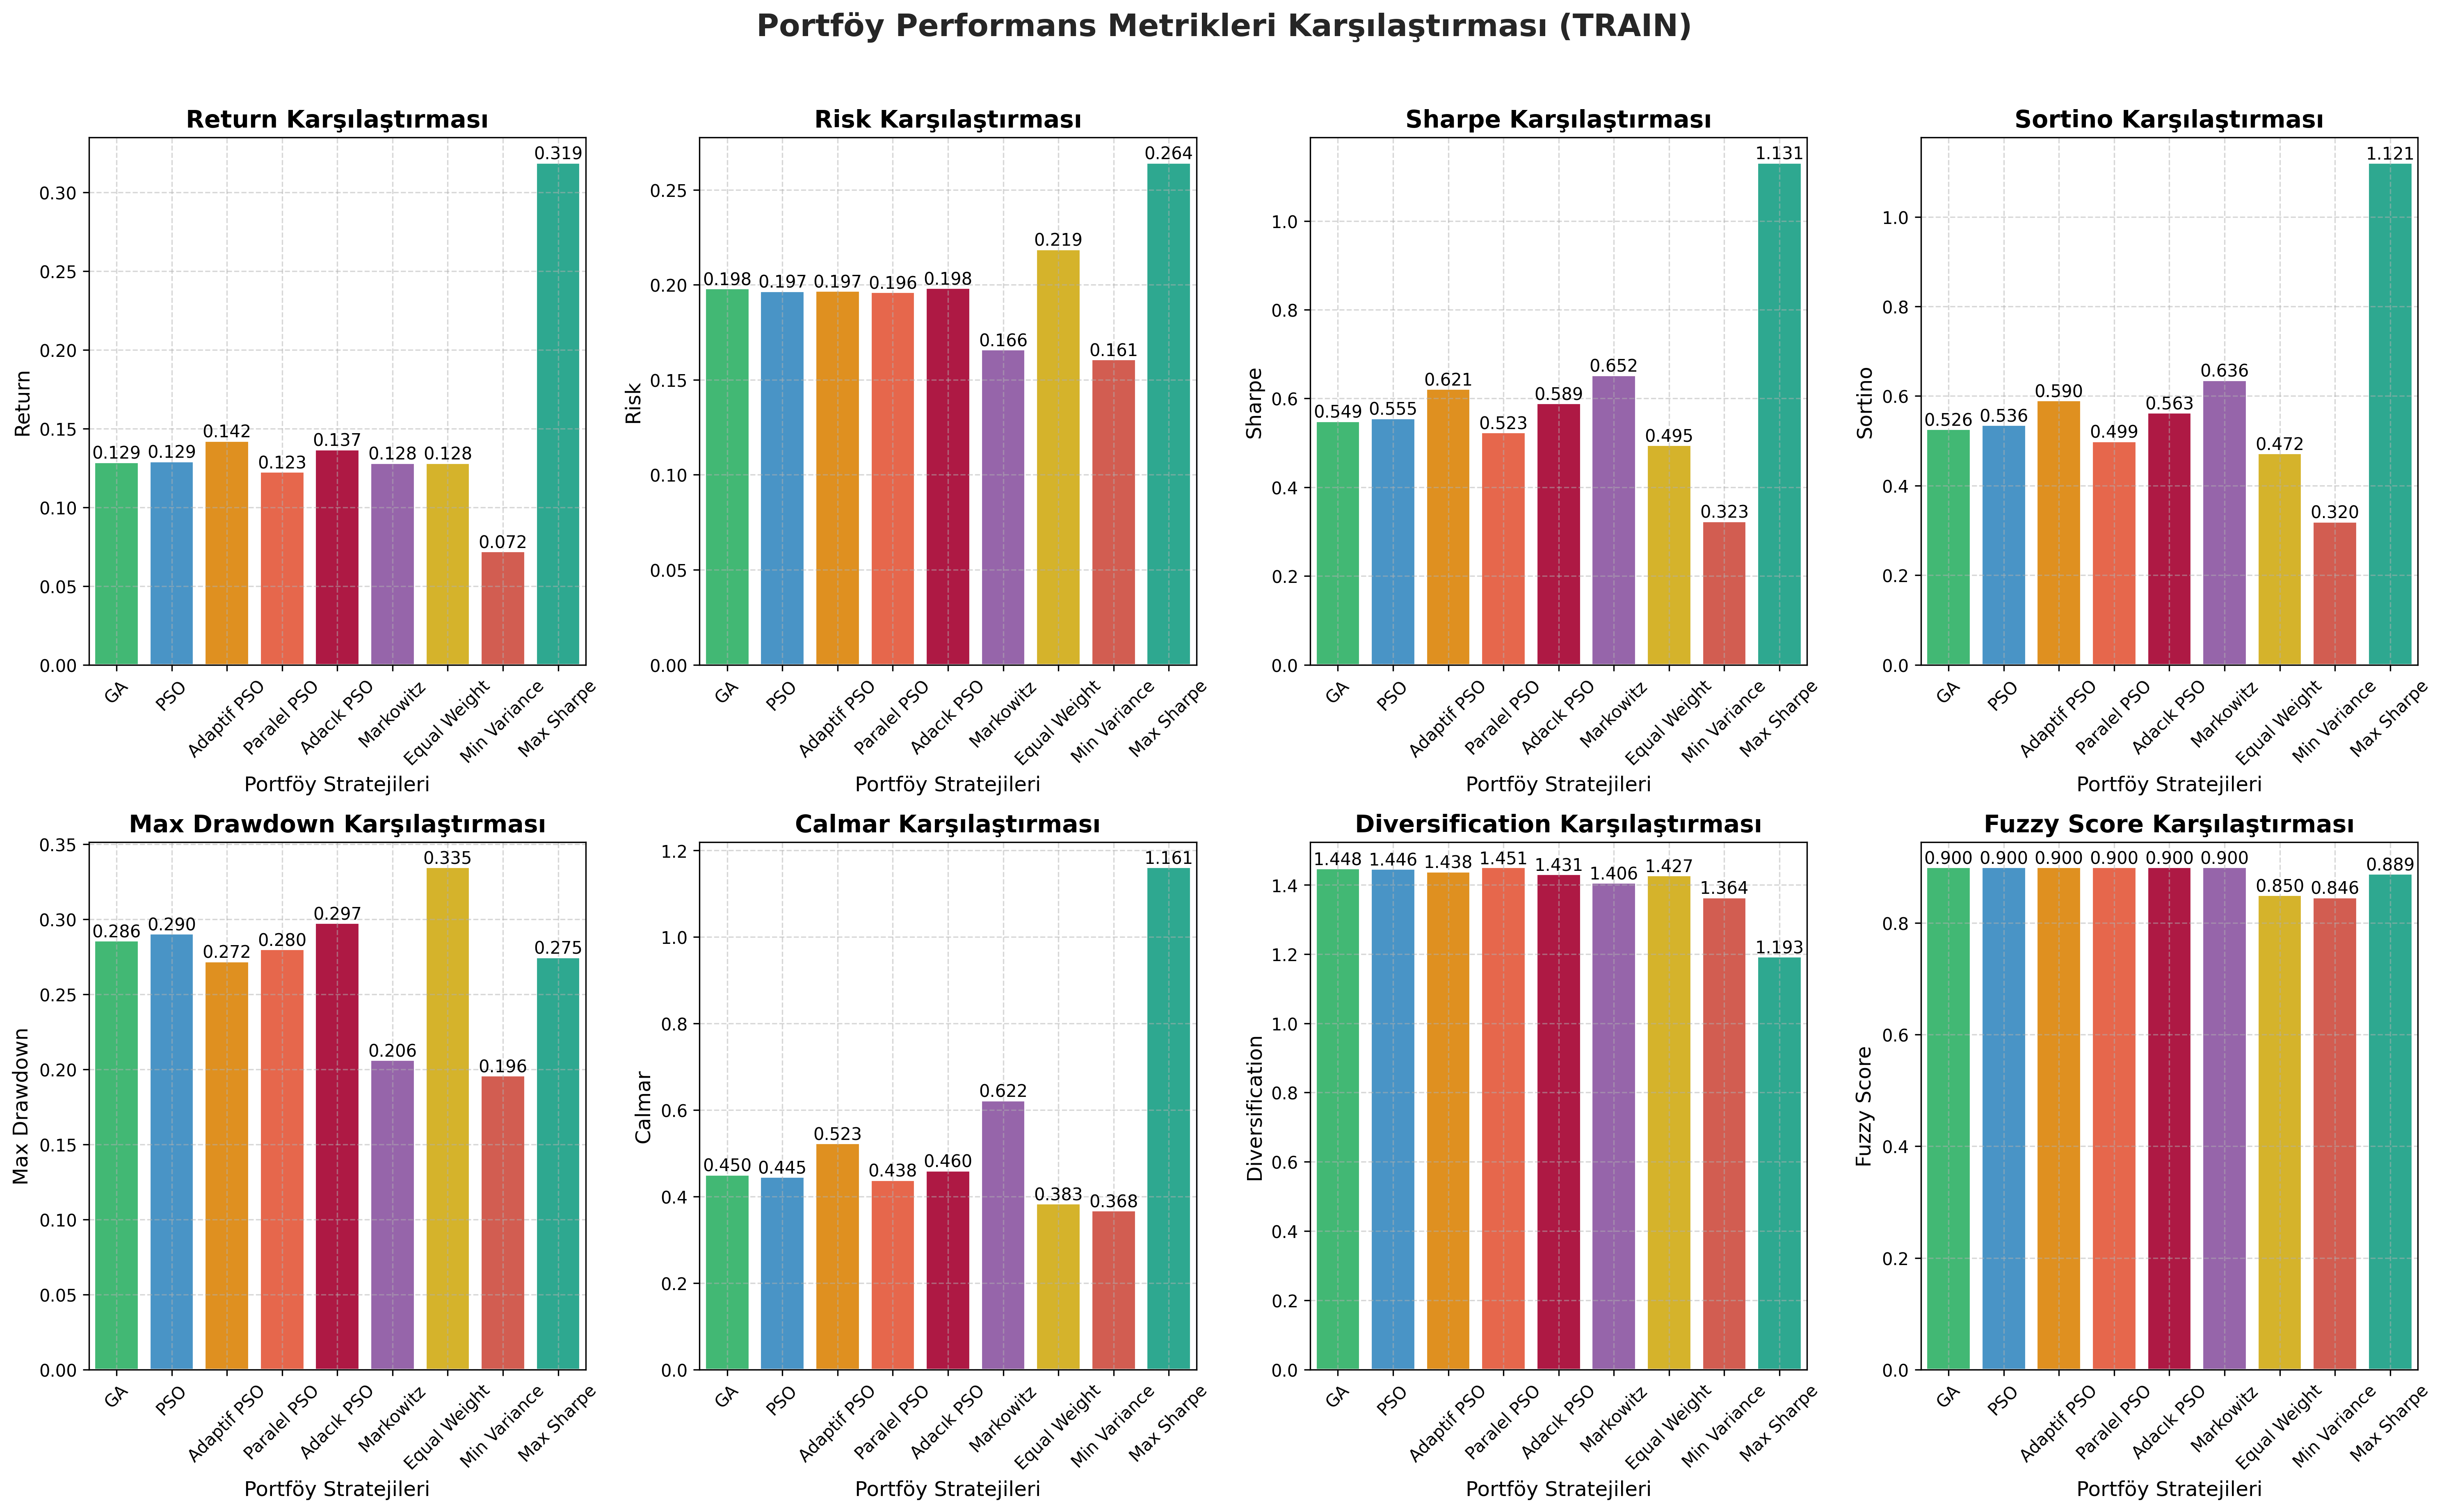
\includegraphics[width=\textwidth, height=5cm, keepaspectratio]{train_performance_metrics_comparison.png}
      % This references the train metrics image you provided
    \end{column}
    \begin{column}{0.48\textwidth}
      \centering
      \textbf{Test Data Metrics}
      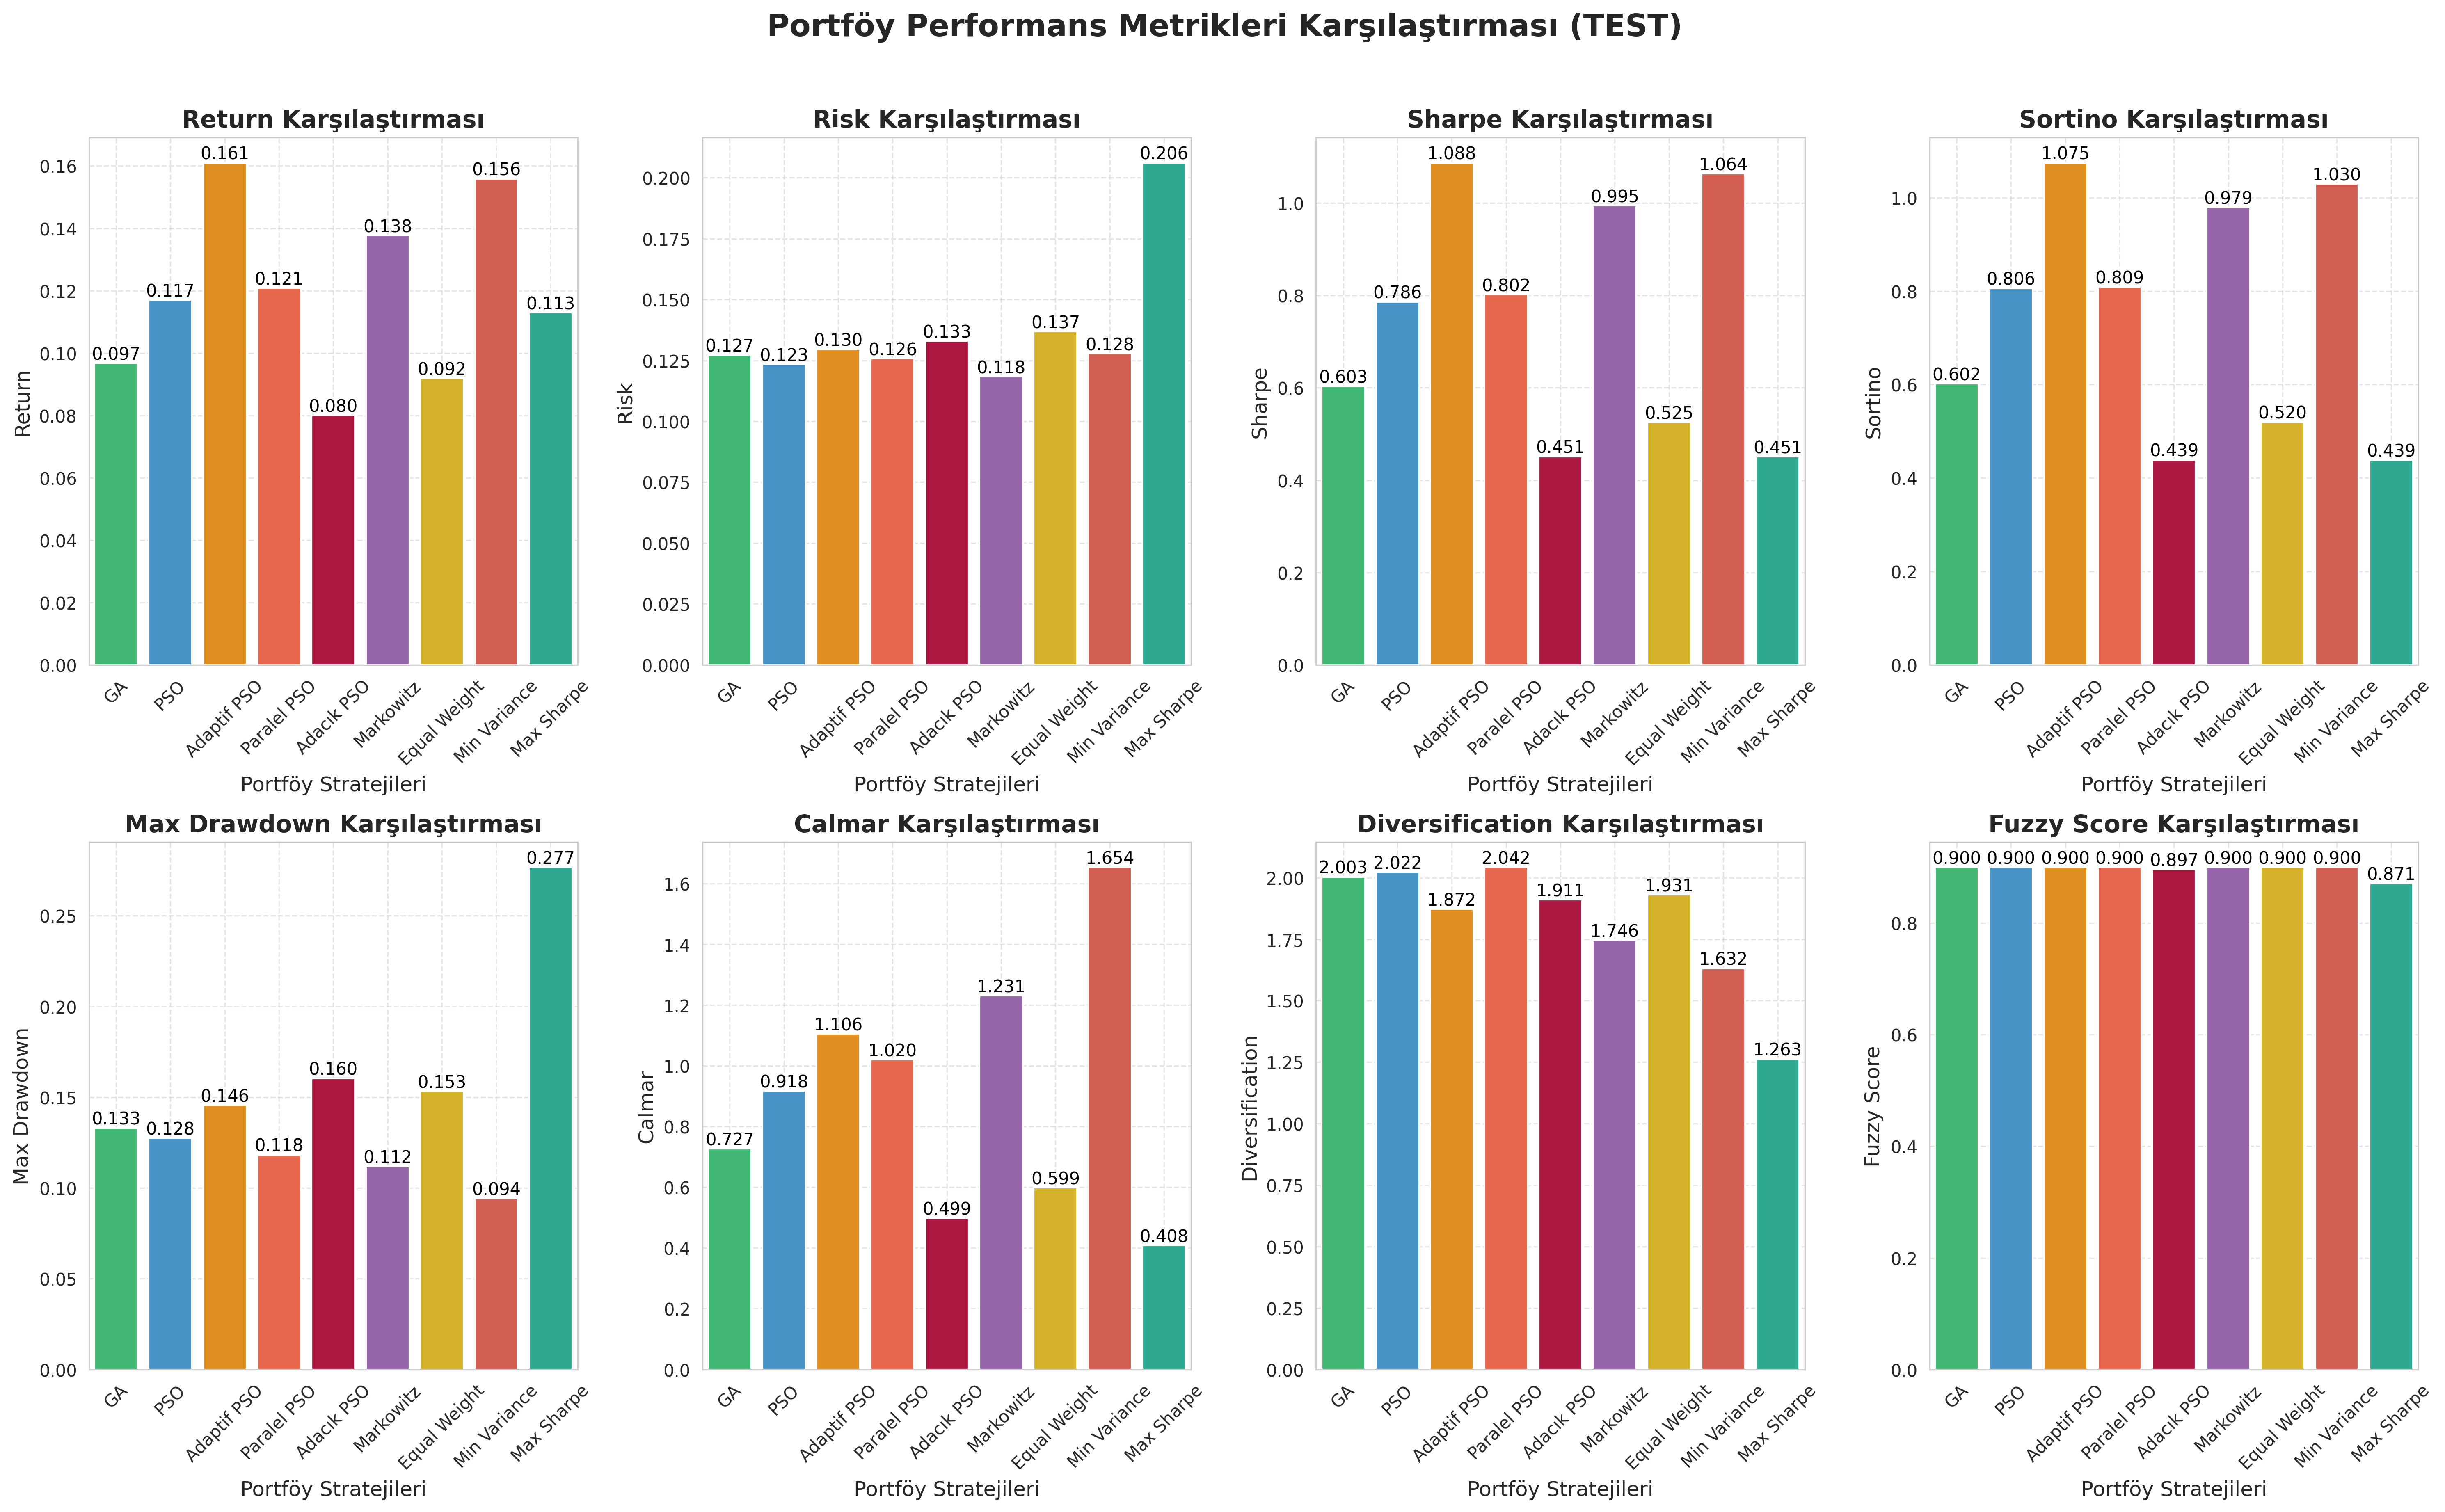
\includegraphics[width=\textwidth, height=5cm, keepaspectratio]{test_performance_metrics_comparison.png}
      % This references the test metrics image you provided
    \end{column}
  \end{columns}
  
  \begin{tcolorbox}[
    enhanced,
    colback=blue!5,
    colframe=blue!70,
    arc=2mm,
    title=Train-Test Performance Analysis,
    fonttitle=\bfseries\large,
    boxrule=0.5mm
  ]
    \begin{itemize}
      \item Max Sharpe showed dramatic overfit (1.131 train vs 0.451 test Sharpe)
      \item Adaptive PSO demonstrated most consistent performance across both datasets
      \item Min Variance had best downside protection in both periods
      \item Island Model PSO performed better in training than testing
    \end{itemize}
  \end{tcolorbox}
\end{frame}

\begin{frame}{Detailed Performance Metrics - Test Data}
  \centering
  \small
  \begin{tabular}{lrrrrrr}
    \toprule
    \textbf{Strategy} & \textbf{Return} & \textbf{Risk} & \textbf{Sharpe} & \textbf{Sortino} & \textbf{Max DD} & \textbf{Calmar} \\
    \midrule
    Adaptive PSO & \textbf{0.1610} & 0.1297 & \textbf{1.0877} & \textbf{1.0749} & 0.1456 & 1.1057 \\
    Min Variance & 0.1559 & 0.1278 & 1.0638 & 1.0296 & \textbf{0.0943} & \textbf{1.6537} \\
    Markowitz    & 0.1377 & \textbf{0.1183} & 0.9948 & 0.9793 & 0.1119 & 1.2308 \\
    Parallel PSO & 0.1208 & 0.1258 & 0.8017 & 0.8092 & 0.1184 & 1.0203 \\
    Standard PSO & 0.1170 & 0.1234 & 0.7863 & 0.8063 & 0.1276 & 0.9175 \\
    GA           & 0.0968 & 0.1272 & 0.6032 & 0.6021 & 0.1331 & 0.7271 \\
    Equal Weight & 0.0919 & 0.1368 & 0.5255 & 0.5199 & 0.1534 & 0.5992 \\
    Island PSO   & 0.0800 & 0.1330 & 0.4514 & 0.4392 & 0.1605 & 0.4988 \\
    Max Sharpe   & 0.1129 & 0.2062 & 0.4507 & 0.4387 & 0.2767 & 0.4082 \\
    \bottomrule
  \end{tabular}
  
  \vspace{0.5cm}
  \begin{tcolorbox}[
    enhanced,
    colback=blue!5,
    colframe=blue!70,
    arc=2mm,
    title=Key Insights,
    fonttitle=\bfseries\large,
    boxrule=0.5mm
  ]
    \begin{itemize}
      \item Adaptive PSO achieved highest risk-adjusted returns (Sharpe and Sortino)
      \item Min Variance strategy provided best downside protection (lowest Max DD)
      \item Markowitz model had lowest risk but moderate return
      \item Traditional Max Sharpe underperformed in the test period due to concentration
      \item More complex algorithms (Island Model) didn't necessarily yield better results
    \end{itemize}
  \end{tcolorbox}
\end{frame}

\begin{frame}{Execution Time Comparison}
  \centering
  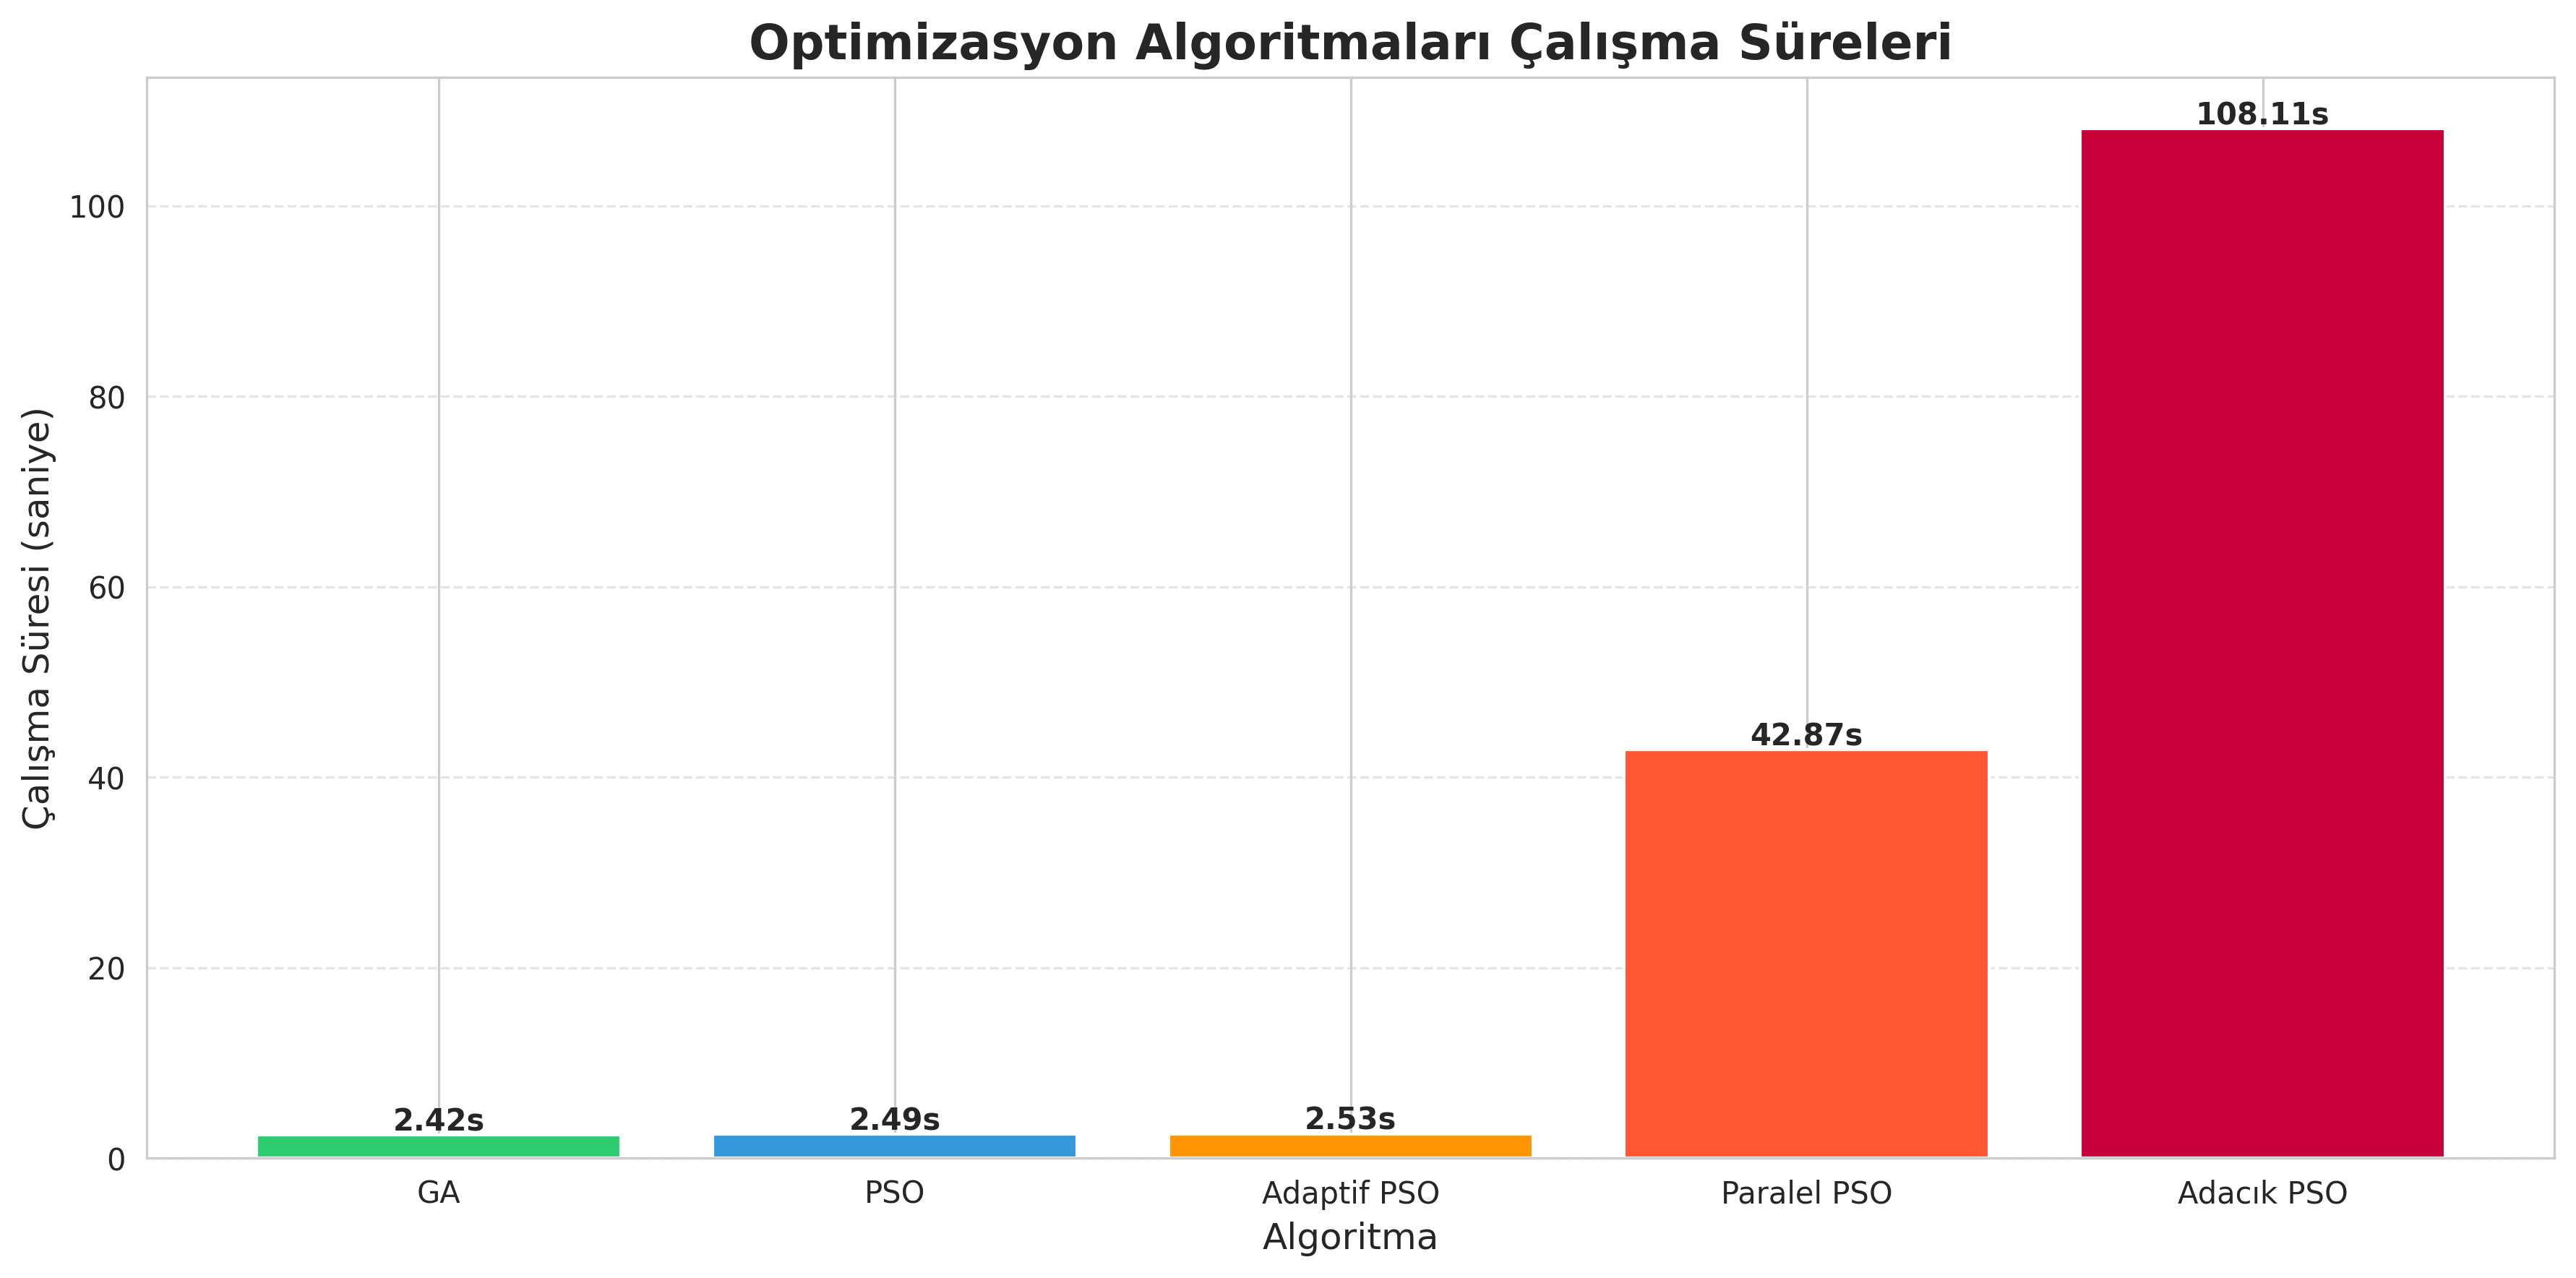
\includegraphics[width=\textwidth, height=5.5cm, keepaspectratio]{execution_times_comparison.png}
  % This shows execution times for all optimization algorithms
  
  \begin{tcolorbox}[
    enhanced,
    colback=blue!5,
    colframe=blue!70,
    arc=2mm,
    title=Performance Analysis,
    fonttitle=\bfseries\large,
    boxrule=0.5mm
  ]
    \begin{itemize}
      \item GA was fastest at 2.42 seconds
      \item Standard PSO (2.49s) and Adaptive PSO (2.53s) comparable
      \item Parallel PSO significantly slower at 42.87 seconds due to overhead
      \item Island Model PSO slowest at 108.11 seconds
      \item Unexpected result: Parallel implementations slower than sequential
      \item Communication overhead and process synchronization dominated execution time
    \end{itemize}
  \end{tcolorbox}
\end{frame}

\begin{frame}{Conclusions}
  \begin{tcolorbox}[
    enhanced,
    colback=blue!5,
    colframe=blue!70,
    arc=2mm,
    title=Key Findings,
    fonttitle=\bfseries\large,
    boxrule=0.5mm
  ]
    \begin{itemize}
      \item Adaptive PSO provides the best balance between performance and computational efficiency
      \item Fuzzy logic guidance helps algorithms find robust portfolios with good out-of-sample performance
      \item Parallel implementations introduce significant overhead that may not be justified for small portfolios
      \item Traditional methods (Markowitz, Min Variance) still perform well but with different risk-return profiles
      \item Parameter adaptation is more effective than increased computational complexity for this problem
    \end{itemize}
  \end{tcolorbox}
  
  \vspace{0.3cm}
  
  \begin{tcolorbox}[
    enhanced,
    colback=green!5,
    colframe=green!70,
    arc=2mm,
    title=Practical Implications,
    fonttitle=\bfseries\large,
    boxrule=0.5mm
  ]
    \begin{itemize}
      \item For portfolio optimization with 30-40 assets, sequential methods are preferable
      \item Adaptive parameter tuning significantly improves optimization quality
      \item Fuzzy logic provides a flexible framework for multi-objective portfolio optimization
      \item Max Sharpe ratio strategies should be carefully examined for overfitting
      \item Min Variance offers good downside protection with competitive returns
    \end{itemize}
  \end{tcolorbox}
\end{frame}

\begin{frame}{Future Research Directions}
  \begin{columns}
    \begin{column}{0.48\textwidth}
      \begin{tcolorbox}[
        enhanced,
        colback=blue!5,
        colframe=blue!70,
        arc=2mm,
        title=Algorithmic Improvements,
        fonttitle=\bfseries\large,
        boxrule=0.5mm
      ]
        \begin{itemize}
          \item Hybrid approaches combining GA and PSO
          \item Quantum-inspired optimization techniques
          \item Deep reinforcement learning for portfolio optimization
          \item Improved island topology and migration policies
          \item Multi-swarm collaborative optimization
        \end{itemize}
      \end{tcolorbox}
    \end{column}
    \begin{column}{0.48\textwidth}
      \begin{tcolorbox}[
        enhanced,
        colback=green!5,
        colframe=green!70,
        arc=2mm,
        title=Application Extensions,
        fonttitle=\bfseries\large,
        boxrule=0.5mm
      ]
        \begin{itemize}
          \item Incorporating ESG criteria in fuzzy framework
          \item Dynamic portfolio rebalancing strategies
          \item Multi-period optimization with transaction costs
          \item Integration with alternative data sources
          \item Risk parity portfolio construction using PSO
        \end{itemize}
      \end{tcolorbox}
    \end{column}
  \end{columns}
  
  \vspace{0.5cm}
  
  \begin{tcolorbox}[
    enhanced,
    colback=yellow!5,
    colframe=yellow!70,
    arc=2mm,
    title=Technical Enhancements,
    fonttitle=\bfseries\large,
    boxrule=0.5mm
  ]
    \begin{itemize}
      \item GPU-based parallel implementation for large portfolios
      \item Improved fuzzy inference systems using type-2 fuzzy logic
      \item Adaptive constraint handling techniques
      \item Distributed computing approaches with optimized communication
      \item Ensemble methods combining multiple optimization strategies
    \end{itemize}
  \end{tcolorbox}
\end{frame}

\begin{frame}{Thank You!}
  \begin{center}
    \Large{Thank you for your attention!}
    
    \vspace{1cm}
    
    \large{Questions?}
    
    \vspace{1cm}
    
    \normalsize{Contact Information:}\\
    Email: cemal.ozturk@pmu.edu.tr\\
    Website: www.pmu.edu.tr/~cemalozturk
  \end{center}
\end{frame}

% References
\begin{frame}[allowframebreaks]{References}
  \begin{thebibliography}{9}
    \bibitem{markowitz} Markowitz, H. (1952).
    \newblock Portfolio Selection.
    \newblock \emph{The Journal of Finance}, 7(1), 77--91.
    
    \bibitem{pso} Kennedy, J., \& Eberhart, R. (1995).
    \newblock Particle swarm optimization.
    \newblock \emph{Proceedings of IEEE International Conference on Neural Networks}, 1942--1948.
    
    \bibitem{adaptive} Shi, Y., \& Eberhart, R. C. (1998).
    \newblock A modified particle swarm optimizer.
    \newblock \emph{IEEE International Conference on Evolutionary Computation}, 69--73.
    
    \bibitem{fuzzy} Zadeh, L. A. (1965).
    \newblock Fuzzy sets.
    \newblock \emph{Information and Control}, 8(3), 338--353.
    
    \bibitem{genetic} Holland, J. H. (1992).
    \newblock Adaptation in natural and artificial systems.
    \newblock \emph{MIT Press}.
    
    \bibitem{parallelPSO} Alba, E., \& Troya, J. M. (2002).
    \newblock Improving flexibility and efficiency by adding parallelism to genetic algorithms.
    \newblock \emph{Statistics and Computing}, 12(2), 91--114.
    
    \bibitem{islandModel} Cantu-Paz, E. (2000).
    \newblock Efficient and accurate parallel genetic algorithms.
    \newblock \emph{Springer Science \& Business Media}.
    
    \bibitem{fuzzyportfolio} Fang, Y., Lai, K. K., \& Wang, S. Y. (2006).
    \newblock Portfolio rebalancing model with transaction costs based on fuzzy decision theory.
    \newblock \emph{European Journal of Operational Research}, 175(2), 879--893.
  \end{thebibliography}
\end{frame}

\end{document}